\documentclass{book}

\usepackage{defs-config-macros}


\begin{document}

\thispagestyle{empty}
\frontmatter
    \begin{minipage}{.3\textwidth}
  \flushleft
  \center{
\includegraphics[scale=.09]{unam.pdf}}

  \vspace{20pt}

  \center{
    \rule{.5pt}{.6\textheight}
    \hspace{7pt}
    \rule{2pt}{.6\textheight}
    \hspace{7pt}
    \rule{.5pt}{.6\textheight}
  } \\

  \center{
\includegraphics[scale=.22]{ciencias.pdf}}
\end{minipage}
\begin{minipage}{.7\textwidth}
\flushright

\center{

  \center{
    \LARGE{U}\large{NIVERSIDAD} \LARGE{N}\large{ACIONAL}
    \LARGE{A}\large{UTÓNOMA} \\[10pt]
    \large{DE}
    \LARGE{M}\large{ÉXICO}
  } \\
  \rule{\textwidth}{2pt}
  \\
  \hrulefill\\[1cm]

  \LARGE{F}\large{ACULTAD DE } \LARGE{C}\large{IENCIAS}\\[2cm]

  \large{
  Análisis del algoritmo \textit{Knuth-Morris-Pratt} con énfasis en la programación funcional
  }\\[1.6cm]

  \huge{
T \hspace{1cm} E \hspace{1cm} S \hspace{1cm} I \hspace{1cm} S  }\\[1cm]

  \large{QUE PARA OBTENER EL TÍTULO DE:}\\[1cm]

  \large{
Licenciado en Ciencias de la Computación  }\\[1cm]

  \large{PRESENTA:}\\[1cm]

  \large{
Ángel Iván Gladín García  }\\[1cm]

  \large{
TUTORA  }\\[.2cm]

  \large{
  Dra. Lourdes Del Carmen González Huesca}\\[1cm]
  \large{
    Ciudad Universitaria, Cd. Mx., 2021
  }
}

\end{minipage}

    \clearpage
    \mbox{}
    \clearpage
    \thispagestyle{empty}
    
    \pagenumbering{Roman} 


\begin{center}
{\Large \textbf{Hoja de Datos del Jurado}}
\vspace*{.85cm}
\end{center}


\begin{enumerate}

\item Datos del Alumno

Gladín \\
García \\
Ángel Iván \\
+52 55 8196 8560 \\
Universidad Nacional Autónoma de México \\
Facultad de Ciencias \\
Ciencias de la Computación \\
313112470


\item Datos de la Tutora

Dra. \\
Lourdes del Carmen \\
González \\
Huesca


\item Datos del Sinodal 1

Dr. \\
Favio Ezequiel \\
Miranda \\
Perea


\item Datos del Sinodal 2

Dra. \\
Adriana \\
Ramírez \\
Vigueras


\item Datos del Sinodal 3

Dr. \\
Canek \\
Peláez \\
Valdés


\item Datos del Sinodal 4

L. en C.C. \\
Fernando Abigail \\
Galicia \\
Mendoza


\item Datos del trabajo escrito

{\small Análisis del algoritmo \textit{Knuth-Morris-Pratt} con énfasis en la programación funcional} \\
100p. \\ % TODO: cambiar el número de hojas
2021 


\end{enumerate} 

    
    \chapter*{Agradecimientos}
    \lipsum[1-2]

    \clearpage
    
    \tableofcontents


\mainmatter
    \chapter*{Motivación y estructura del trabajo}
        En mi camino aprendiendo y escribiendo programas usando programación funcional, es algo común ver un programa
que aunque sea corto y legible, muchas veces es algo ineficiente. Entonces es ahí cuando Richard Bird tiene
en mente que un programa debe actuar como la especificación formal del problema, pero también por medio del
razonamiento ecuacional poder calcular uno más eficiente.
Uno de los factores que ayudó al crecimiento en el interés de la programación funcional, fue que en los años
1990's se dieron cuenta que estos lenguajes son buenos para hacer razonamiento ecuacional.
De hecho el lenguaje funcional Gofer, inventado por Mark Jones capturó este pensamiento como un acrónimo 
(\textit{Good for equational reasoning}).
\newline

Lo que se abordará en este trabajo es primero empezar con una especificación en Haskell y después proseguir a
calcular una versión más eficiente por medio de razonamiento ecuacional.
La razón de este trabajo es ver hasta donde el diseño de un algoritmo puede estar encajado en una forma
matemática de calcular un resultando usando principios matemáticos bien establedicos como definiciones, 
teoremas, y \textit{``leyes''}.
Curiosamente, es generalmente verdadero que en matemáticas los cálculos están diseñados para simplificar
cosas complicadas, en el diseño de algoritmos usualmente es al revés.
\begin{quote}
Simples, pero ineficientes programas son transformados en versiones más eficientes que puedes ser
completamente opacas en su implementación.
\end{quote}
Explicando las ideas detrás de un algoritmo es mucho más fácil en un estilo funcional, en vez de un
procedimental. Las funciones pueden ser separadas fácilemente, cada una es sucinta y capturan patrones
de cómputo.
\newline

Los algoritmos de búsqueda de subcadenas (\textit{String Matching Algorithms}) son usados frecuentemente en:
programas de edición de texto para encontrar todas las ocurrencias de un patrón en un texto, para encontrar
patrones particulares en una cadenas de ADN, o también en algunos motores de búsqueda los utilizan para
encontrar páginas web en búsquedas, entre otras aplicaciones. Algoritmos efecientes para atacar este tipo de
problemas nos ayudan gratamente para mejorar el tiempo de la búsqueda.
\newline

TODO
    \addcontentsline{toc}{chapter}{Motivación y estructura del trabajo}
    
    \chapter{Fundamentos}
        En este capítulo se verá como, dado un conjunto de definiciones de funciones, por medio de razonamiento ecuacional podemos llegar a otras definiciones y/o probarlas. Las pruebas aquí se harán mediantte inducción.

Muchas veces es algo engorroso probar funciones similares repetidamente, por eso veremos una forma de hacer pruebas (en algunos casos) más cortas,
presentando unas \textit{funciones de orden superior} que encapsulan patrones comunes de cómputo. Y así, probar resultados más generales y apelar a ellos.

Al final se verá que la eficiencia también importa, porque se mostrarán algunos ejemplos; como un problema famoso llamado \textit{``The maximum segment sum''}
y una mejora de la función \texttt{scanr}. Y todo esto se logrará como consecuencia de lo dicho anteriormente.

\subsection{Inducción sobre listas}
Recordemos que toda lista finita es de la forma; una lista vacía \texttt{[]} ó \texttt{x:xs} donde \texttt{xs} es una lista finita. Por consiguiente, para probar que $P(xs)$ se mantiene para todas las lista finitas $xs$,
se tiene que probar que:

\begin{enumerate}
    \item $P([])$ se cumple
    \item Para toda $x$ y para todas las listas finitas $xs$, que $P(x:xs)$ se cumple dado que $P(xs)$ también.
\end{enumerate}

Tomemos la definición de concatenación \texttt{(++)},
\inputminted{haskell}{definiciones/concatenation.hs}

Y ahora probemos que (++) es asociativa para todas las listas finitas $xs$, es decir:

(xs ++ ys) ++ zs = xs ++ (ys ++ zs)

Por inducción sobre $xs$:

%{\displaystyle x+5} is the left-hand side (LHS) and {\displaystyle y+8}{\displaystyle y+8} is the right-hand side (RHS).
%FIXME: si caben dos eucaciones por lado lo hago en columnas.

\begin{itemize}
\item Caso []
\begin{minted}{haskell}
(LHS)

([] ++ ys) ++ zs
=   {++.1}
ys ++ zs
\end{minted}

\begin{minted}{haskell}
(RHS)

[] ++ (ys ++ zs)
=   {++.1}
ys ++ zs
\end{minted}

\item Caso (x:xs)
\begin{minted}{haskell}
(LHS)

((x:xs) ++ ys) ++ zs
=   {++.2}
(x:(xs ++ ys)) ++ zs
=   {++.2}
x:((xs ++ ys) ++ zs)
\end{minted}

\begin{minted}{haskell}
(RHS)

(x:xs) ++ (ys ++ zs)
=   {++.2}
x:(xs ++ (ys ++ zs))
=   {induction}
x:((xs ++ ys) ++ zs)
\end{minted}

\end{itemize}

\subsection*{La función \texttt{foldr}}
\subsection*{La función \texttt{scanl}}

\begin{minted}{haskell}
scanl (@) e [x, y, z, ...] = [e, e@x,(e@x)@y,((e@x)@y)@z,...]

\end{minted}



\section{Programación funcional}
De forma muy general y resumiendo, la programación funcional:
\begin{itemize}
    \item es un método de construcción de un programa que hace énfasis en las funciones y sus aplicaciones
    en vez de cómandos y sus ejecuciones.

    \item usa notación matemática simple que permite que los problemas sean descritos de manera clara
    y consisa.
    \item tiene bases matemáticas que fundamentan el razonamiento ecuacional acerca de las propiedades de
    los programas.
\end{itemize}

\section{Definiciones inductivas y recursivas}
%TODO

\section{Razonamiento ecuacional}
%TODO


\section{Definiciones de listas}
%TODO

\section{Principio de Fusión}
\begin{minted}{haskell}
f . foldr g a = foldr h b
\end{minted}

\begin{itemize}
    \item $f$ es una función estricta.
    \item $f a = b$
    \item $f(g y x) = h (f y) x$ para toda $x$ y $y$.w
\end{itemize}

\section{\textit{The maximum segment sum}}

    
    \chapter{Análisis de tiempo}
        \lipsum[1-1]

\section{Notación asintótica}
%TODO

\section{Estimando tiempo}
%TODO

\section{Tiempo amortizado}
%TODO

    
    \chapter{Algoritmos de búsqueda de subcadenas}
        En diversas situaciones se necesita encontrar todas las ocurrencias de un patrón en un texto;
éstas pueden ir desde editores de texto hasta buscar patrones particulares en secuencias de ADN.
Es aquí cuando se hace uso de algoritmos eficientes para este problema.

Es aquí cuando se formaliza el problema de ``búsqueda de subcadenas'' (string-matching).
Supongamos que el texto es un arreglo $T[1 \ldots n]$ de longitud $n$ y el patrón es un arreglo
$P[1 \ldots m]$ de longitud $m \leq n$. También supongamos que los elementos de $P$ y $T$ son
caracteres tomados de un alfabeto finito $\Sigma$. El arreglo de caracteres $P$ y $T$ también son
llamados \textbf{cadenas} de caracteres.

\section{Notación y terminología}

Decimos que el patrón $P$ \textbf{ocurre con un desplazamiento} $s$ en el texto $T$ si
$0 \leq s \leq n - m$ y $T[s+1 \ldots s+m] = P[1 \ldots m]$. Si $P$ ocurre con un desplazamiento
$s$ en $T$, entonces se dice que $s$ es \textbf{un desplazamiento válido}, si no, se dice que $s$
es \textbf{un desplazamiento inválido}.
El \textbf{problema de búsqueda de subcadenas} es el problema de encontrar todos los
desplazamientos válidos en los que dado el patrón $P$ ocurre en el ttexto $T$.

% aquí poner la imagen del la figura 32.1 y explicarlo

Denotemos a $\Sigma^*$ como el conjunto de todas las cadenas de longitud finita formadas usando
caracteres del alfabeto $\Sigma$. La cadena de longitud cero es \textbf{la cadena vacía}, denotada
como $\varepsilon$, que también pertenece a $\Sigma^*$. La longitud de una cadena $x$ se denota
como $\vert x \vert$. La \textbf{concatenación} de dos cadenas $x$ y $y$, se denota como $xy$ y
tiene como longitud $\vert x \vert + \vert y \vert$ y consiste de los caracteres de $x$ seguidos
por los caracteres de $y$.

Decimos que una cadena $w$ es \textbf{prefijo} de una cadena $x$, denotada como $w \sqsubset x$, si
$x = wy$ para alguna cadena $y \in \Sigma^*$. Notemos que si $w \sqsubset x$, entonces
$\vert w \vert \leq \vert x \vert$. De manera análoga, decimos que una cadena $w$ es \textbf{sufijo}
de una cadena $x$, denotado como $w \sqsupset x$, si $x = yw$ para alguna $y \in \Sigma^*$. Y así
como con el prefijo, si $w \sqsubset x$, entonces $\vert w \vert \leq \vert x \vert$.
Por ejemplo, tomemos \texttt{ab $\sqsubset$ abcca} y \texttt{cca $\sqsupset$ abcca}. La cadena
vacía $\varepsilon$ es tanto un sufijo coomo un prefijo para cualquier cadena.

\section{Algoritmo de búsqueda de subcadenas ingenuo (\textit{naïve})}

\begin{algorithm}[H]
    \SetKwProg{Fn}{NAIVE-STRING-MATCHER($T,P$)}{}{}
    \Fn{}{
        $n = T.length$\\
        $m = T.length$\\
        \For{$s = 0 $ \KwTo $n-m$}{
            \If{$P[1\ldots m] == T[s+1 \ldots s+m]$}{
                $print$ ``Pattern occurs with shift'' $s$
            }
        }
    }
\end{algorithm}

\section{Algoritmo Knuth-Morris-Prattt}
% TODO: ver qué agarro de aquí: https://en.wikipedia.org/wiki/Knuth%E2%80%93Morris%E2%80%93Pratt_algorithm

\subsection{Diferencias entre KMP Y MP}
% TODO: https://www.cs.helsinki.fi/u/tpkarkka/teach/14-15/SPA/lecture04.pdf
% https://studylib.net/doc/7580926/chapter-6-the-mp-and-kmp-algorithms--algorithms-based-upon

% http://www-igm.univ-mlv.fr/~lecroq/string/node7.html#SECTION0070
%http://www-igm.univ-mlv.fr/~lecroq/string/node8.html

\begin{algorithm}[H]
    \SetKwProg{Fn}{KMP-MATCHER($T,P$)}{}{}
    \Fn{}{
        $n = T.length$\\
        $m = T.length$\\
        $\pi =$ COMPUTE-PREFIX-FUNCTION($P$)\\
        $q = 0$\\    
        \For{$i = 1 $ \KwTo $n$}{
            \While{$q >0$ and $P[q+1] \neq T[i]$}{
                $q = \pi[q]$
            }
            \If{$P[q+1] == T[i]$}{
                $q = q + 1$
            }
            \If{$q == m$}{
                $print$ ``Pattern occurs with shift'' $i-m$\\
                $q = \pi[q]$
            }
        }
    }
\end{algorithm}


\begin{algorithm}[H]
    \SetKwProg{Fn}{COMPUTE-PREFIX-FUNCTION($P$)}{}{}
    \Fn{}{
        $m = P.length$\\
        let $\pi[1 \ldots m]$ be a new array\\
        $\pi[1] =0$\\
        $k = 0$\\    
        \For{$q = 2 $ \KwTo $m$}{
            \While{$k >0$ and $P[k+1] \neq P[q]$}{
                $k = \pi[k]$
            }
            \If{$P[k+1] == P[q]$}{
                $k = k + 1$
            }
            $\pi[k] = k$
        }
        \Return $\pi$
    }
\end{algorithm}

En un capítulo posterior se atacará este problema resulto en Haskell y C++ %% TODO: poner liga al capítulo
%% KMP
% TODO: poner liga al cormen
% TODO: cormen respuestas https://walkccc.me/CLRS/Chap32/32.4/

\begin{tcolorbox}
%% SUFFIX FUNCTION
32.4-1
Compute the prefix function $\pi$ for the pattern \texttt{ababbabbabbababbabb}.
\end{tcolorbox}

\begin{tcolorbox}
\hypertarget{cyclic_rotation}{32.4-7}
Give a linear-time algorithm to determine whether a text $T$ is a cyclic rotation of another string
$T'$ . For example, \texttt{arc} and \texttt{car} are cyclic rotations of each other.
\end{tcolorbox}

\begin{tcolorbox}
\hypertarget{repetition_factor}{32.1 a.}
\textbf{String matching based on repetition factors}
Let $y^i$ denote the concatenation of string y with itself $i$ times. For example,
\texttt{ab}$^3 =$ \texttt{ababab}. We say that a string $x \in \Sigma^*$
\textbf{has repetition factor} $r$ if $x = y^r$ for some string $y \in \Sigma^*$ and some $r > 0$.
Let $\rho(x)$ denote the largest $r$ such that $x$ has repetition factor $r$.
a. Give an efficient algorithm that takes as input a pattern $P[1 \ldots m]$ and computes the value
$\rho(x)$ for $i = 1,2,\ldots,m$. What is the running time of your algorithm?
\end{tcolorbox}

\section{Diferentes tipos de algoritmos en cadenas}


    \chapter{Función de error}
        En este capítulo se derivará por medio de una especificación formal la función de error del
algoritmo de KMP. Aunque por medio de este acercamiento\cite{bird:cyclic} se podría obtener todo
el algoritmo KMP usando estructuras cíclicas, específicameente listas doblemente ligadas, no se
hará así, porque se verá otra manera ``puramente funcional'' de hacerlo en el siguiente capítulo.

Consideremos la cadena \texttt{abacabab} y su procesamiento con la función de error,

\begin{table}[h]
\centering
\begin{tabular}{c|c|c|c|c|c|c|c|c|}
\cline{2-9}
$k$      & 1          & 2          & 3          & 4          & 5          & 6          & 7          & 8          \\ \hline
$P[k]$   & \texttt{a} & \texttt{b} & \texttt{a} & \texttt{c} & \texttt{a} & \texttt{b} & \texttt{a} & \texttt{b} \\ \hline
$\pi[k]$ & 0          & 0          & 1          & 0          & 1          & 2          & 3          & 2          \\ \cline{2-9} 
\end{tabular}
\end{table}

La entrada $\pi[k]$ en la posición $b$ es la longitud del \textbf{sufijo propio más largo} de
\hsCode{take k "abacabab"} que también es un prefijo de \hsCode{"abacabab"}.

Veamos del procesamiento de la cadena de arriba:
\begin{itemize}
\item[$\pi{[1]}$] Dado que el sufijo propio más largo de \hsCode{take 1 "abacabab" = "a"} es
$\varepsilon$, siempre la primera posición será 0. Por lo que $\pi[1] = 0$.
\item[$\pi{[2]}$] El sufijo propio más largo de \hsCode{take 2 "abacabab" = "ab"} que también es
prefijo de \texttt{abacabab} es $\varepsilon$. Por lo que $\pi[2] = 0$.
\item[$\pi{[3]}$] El sufijo propio más largo de \hsCode{take 3 "abacabab" = "aba"} que también es
prefijo de \texttt{abacabab} es \texttt{a}. Por lo que $\pi[3] = 1$.
\item[$\pi{[4]}$] El sufijo propio más largo de \hsCode{take 4 "abacabab" = "abac"} que también es
prefijo de \texttt{abacabab} es $\varepsilon$. Por lo que $\pi[4] = 0$.
\item[$\pi{[5]}$] El sufijo propio más largo de \hsCode{take 5 "abacabab" = "abaca"} que también
es prefijo de \texttt{abacabab} es \texttt{a}. Por lo que $\pi[5] = 1$.
\item[$\pi{[6]}$] El sufijo propio más largo de \hsCode{take 6 "abacabab" = "abacab"} que también
es prefijo de \texttt{abacabab} es \texttt{ab}. Por lo que $\pi[6] = 2$.
\item[$\pi{[7]}$] El sufijo propio más largo de \hsCode{take 7 "abacabab" = "abacaba"} que también
es prefijo de \texttt{abacabab} es \texttt{aba}. Por lo que $\pi[7] = 3$.
\item[$\pi{[8]}$] El sufijo propio más largo de \hsCode{take 8 "abacabab" = "abacabab"} que también
es prefijo de \texttt{abacabab} es \texttt{ab}. Por lo que $\pi[8] = 2$.
\end{itemize}

Para una lista no vacía \texttt{as}, los sufijos \textbf{propios} de \hsCode{take k as} son sufijos
de \hsCode{take (k-1) (tail as)}, el $k-1$ es porque como se afirma que la lista \texttt{as} es no
vacía, se contemplan en los sufijos propios a la lista vacía, y a \hsCode{tail as} de manera
similar.

Teniendo así una forma de calcular todos los sufijos \textbf{propios} de una lista \texttt{as} como:
\begin{minted}{haskell}
[take (k - 1) (tail as) | k <- [1 .. length as]] = inits (tail as)
\end{minted}

De igual manera se mostrará por medio de un ejemplo concreto tales sufijos propios,
\begin{minted}{haskell}
>>> inits (tail "abacabab")
    inits "bacabab"
    ["","b","ba","bac","baca","bacab","bacaba","bacabab"]
\end{minted}

donde \hsCode{inits}\footnote{
    La función \hsCode{inits} viene definida en el módulo \hsCode{Data.List}.
    }
regresa una lista con los prefijos de una lista en orden creciente y \hsCode{tail} extrae la cabeza
de la lista.

La función de error se define como:
\inputminted[fontsize=\small]{haskell}{codigo/haskell/FailureFunctionNaive.hs}

Donde \hsCode{llasp as bs} es la longitud del sufijo más largo de \texttt{bs} que es también un
prefijo de \texttt{as}. Esto es porque la función \hsCode{tails}\footnote{
    La función \hsCode{tails} viene definida en el módulo \hsCode{Data.List}.
    }
regresa todos los sufijos en orden decreciente y con la función \hsCode{head} solo se obtiene el
primero (que evidentemente es el mayor). Y así \hsCode{ptable} calcula la función de error como
una lista.

Si se calcula \hsCode{ptable "abacabab"} el resultado es:
\begin{minted}{haskell}
>>> ptable "abacabab"
    [(1,('a',0)),(2,('b',0)),(3,('a',1)),(4,('c',0)),(5,('a',1)),
     (6,('b',2)),(7,('a',3)),(8,('b',2))]
\end{minted}

Recordando el \textit{Scan Lemma}\ref{fundamentos:scan_lemma} y viendo que hay un \hsCode{inits} en
\hsCode{ptable} veamos si se puede optimizar. El \textit{Scan Lemma} afirma que
\begin{minted}{haskell}
map (foldl op e) . inits = scanl op e
\end{minted}

Para expresar a \hsCode{llasp as bs} en la forma de un pliegue \hsCode{foldl (op as) e} se debe
demostrar que: % TODO: The universal property of fold

\begin{minted}{haskell}
llsap as []          = e
llsap as (bs ++ [b]) = op as (llsap as bs) b
\end{minted}
Para una definición adecuada de \hsCode{e} y \hsCode{op}. 

Es inmediato que \hsCode{llsap as [] = 0} porque el sufijo \texttt{[]} que es prefijo de
\texttt{as} es de longitud 0 y así \texttt{e = 0}.

Lo interesante es encontrar \hsCode{op}. Sea\hsCode{ k = llsap as bs} donde \texttt{k} y\\
\hsCode{ a = head (drop k as)}, así \texttt{a} es el siguiente elemento de \texttt{as} después del
prefijo más largo de \texttt{as} que se empareja con el sufijo de \texttt{bs}.

Para ejemplificarlo consideremos los siguientes ejemplos sobre la cadena original \texttt{abacabab}.
\begin{itemize}
\item Consideremos $i = 3$ donde\hsCode{ bs = take 3 "abacabab" = "aba"},\\
\hsCode{llsap "abacabab" "a" = 1}\\
\hsCode{head (drop 1 "abacabab") = head "bacabab" = 'b' = a}.
Y así \texttt{a\colorbox{yellow}b}\texttt{acabab}.
\item Consideremos $i = 6$ donde\hsCode{ bs = take 6 "abacabab" = "abacab"},\\
\hsCode{llsap "abacabab" "ab" = 2}\\
\hsCode{head (drop 2 "abacabab") = head "acabab" = 'a' = a}.
Y así \texttt{ab\colorbox{yellow}a}\texttt{cabab}.
\end{itemize}

Si \texttt{a = b}, entonces \hsCode{llsap as (bs ++ [b]) = k+1} porque % TODO: explicar

Si no, \texttt{k = 0} entonces \hsCode{llsap as (bs ++ [b]) = 0} porque % TODO: porque no hay sufifo que sea prefijo

En el caso que queda se tiene % TODO: explicar que es porque, pero en sí es porque es un segmento de bs es un segmento de take (k-1) as
\begin{minted}{haskell}
llsap as (bs ++ [b]) = llsap as (take (k - 1) (tail as) ++ [b])
\end{minted}

Así \texttt{llasp as bs = foldl (op as) bs}, donde
\begin{minted}{haskell}
op as k b  | a == b    = k + 1
           | k == 0    = 0
           | otherwise = llsap as (take (k - 1) (tail as) ++ [b])
               where a = head (drop k as)
\end{minted}

% TODO: quitar esto de los backpointers, es más ni lo usi
Ahora viene la parte donde la representación de la tabla de apuntadores \textit{back} como un arreglo en vez de una lista
resulta útil. Poniendo \texttt{xa = ptable as}, se puede ver que,

% TODO: decir que aquí usaré ya arrays
\begin{minted}{haskell}
head (drop k as)                        = fst (xa!(k + 1))
llsap as (take (k - 1) (tail as) ++ [b] = op as (llsap as (take (k - 1) (tail as))) b
                                        = op as (snd (xa!k)) b
\end{minted}

% TODO: poner paso intermeedio de lista a arreglo.
Recordando que \hsCode{xa} es 1-indexada. Esto significa que \hsCode{ptable} queda redefinida como


\inputminted{haskell}{codigo/haskell/FailureFunctionOptimized.hs}


    \chapter{Algoritmo Knuth-Morris-Pratt}
        \section{Planteamiento y algunas observaciones}

Como ya hemos explicado anteriormente, el problema de \textit{string matching} se trata de buscar
todas las ocurrencias de una cadena no vacía, que se le denominará \textbf{patrón} en una cadena
llamada \textbf{texto}. 

La terminología usada en todo este capítulo será:
\begin{itemize}
    \item \texttt{ws} que denotará al patrón y
    \item \texttt{xs} el texto.
\end{itemize}

Como se mencionó en la motivación de este trabajo, lo que se hará es dar una especificación en
Haskell para después irlo ``mejorando''. Empecemos con esta especificación,

\begin{minted}{haskell}
matches :: Eq a => [a] -> [a] -> [Int]
matches ws = map length . filter (endswith ws) . inits  -- (ec.91)
\end{minted}

% TODO, explicar filter, length y map. Al final la composición de todo

La función \hsCode{inits} regresa una lista con los prefijos de una lista en orden creciente como se 
puede ver a continuación,

\begin{minted}{haskell}
>>> inits [2,3,5]
    [[],[2],[2,3],[2,3,5]]
\end{minted}

Donde \hsCode{inits} está definida como:

\inputminted{haskell}{definiciones/inits.hs}

La función \hsCode{endswith ws xs} verifica si el patón \texttt{ws} es sufijo de \texttt{xs}. Más adelante esta función será definida formalmente.

El valor de \hsCode{matches ws xs} es una lista de enteros $p$ tal que \texttt{ws} es un sufijo de \hsCode{take p xs}. Por ejemplo

\begin{minted}{haskell}
>>> matches "abcab" "ababcabcab" 
    [7, 10]
\end{minted}

En otras palabra, \hsCode{matches ws xs} regresa una lista de enteros donde cada entero $p$ indica que
\texttt{ws} aparece en \texttt{xs} terminando en la posición $p$ (siendo 1-indexado).

La función \hsCode{matches} es polimórfica, así que cualquier algoritmo del problema tiene que
depender de la función de comparación \hsCode{(==) :: a -> a -> Bool} sobre elementos de dos listas.
Asumiendo que toma tiempo constante hacer la función de comparación, la complejidad en tiempo de
\hsCode{matches ws xs} es de $\Theta(mn)$ pasos en el peor de los casos, donde $m$ el la longitud de \texttt{ws} y $n$ la
de \texttt{xs}.

Nuestra meta aquí es deerviar el algoritmo KMP para emparejamiento de cadenas, el cual reduce el tiempo a $\Theta(m+n)$ pasos.
Y aquí el ``truco'' a utilizar es aplicar estrategias como leyes de fusión, tuple %% poner todas las estrategias que usaré
para poder manipular la expresión %% TODO: aquí es donde tengo que poner las venttajas de la programación funciional y su manipulación algebraica.

Así un emparejamiento (\textit{match}) ocurre en la posición $p$ si el patrón \texttt{ws} aparece en el texto \texttt{xs} terminando en $p$.


Siempre hay que tener en cuenta que cualquier problema que involucre la función \hsCode{inits}, la ley más importante es conocida como \textbf{Scan Lemma}: %% TODO: referirme al capittulo donde demuestre esto
\begin{minted}{haskell}
map (foldl op e) . inits = scanl op e  -- (ec.92)
\end{minted}

¿Por qué usar \textbf{Scan Lemma}? En pocas pabras para mejorar la complejidad en tiempo evaluando menos expresiones.
Porque en (ec.92), en la expresión LHS es evaluado en una lista de longitud $n$ con $\Theta(n^2)$ evaluaciones de \hsCode{op}, mientras que
en RHS en la expresión equivalente en la función estándar de Haskell \hsCode{scanl} solo requiere $\Theta(n)$ evaluaciones.

Aunque hay un \hsCode{map} en la definición de \hsCode{matches}, también hay un \hsCode{filter}, así que el primer paso en tranformar \hsCode{matches} is reescribir la especificación usando otra ley: %% TODO: hacer una referencia a esta ley y demostrarla

\begin{minted}{haskell}
map f . filter p = map fst . filter snd . map (fork (f,p))  -- (ec.93)
\end{minted}

donde \hsCode{fork (f, p) x = (f x, p x)}. La ley usada simplemente es para poner a \hsCode{map}
después de \hsCode{inits} para prepararlo para aplicar el \textit{scan lemma}. Usando (ec.93) nos lleva a

\begin{minted}{haskell}
matches ws
  = map length . filter (endswith ws)  -- (ec.91)
  = map fst . filter snd . map (fork (length , endswith ws)) . inits  -- Por (e.93)
\end{minted}

La siguiente pregunta a responder es: ¿Puede \hsCode{fork (length, endswith ws)} puede ser convertido
como una instancia de \hsCode{fold}? Ciértamente \hsCode{length = foldl count 0} donde
\hsCode{count n x = n + 1} % TODO: Detallar aquí porqué, caso base e inducción 
Ahora veamos como podemos escribir a \hsCode{endswith ws} como una instancia de \hsCode{foldl}.
Supongamos que se pueden encontrar \hsCode{e} y \hsCode{op}, los cuales dependen de \texttt{ws} tal que,

\begin{minted}{haskell}
endswith ws = foldl op e  -- (ec.94)
\end{minted}

Entonces estamos en posición de aplicar otra ley: la \textit{tupling law} para \hsCode{foldl}. La ley establece que,

\begin{minted}{haskell}
fork (foldl op1 e1, foldl op2 e2) = foldl op (e1, e2)  -- (ec.95)
\end{minted}

donde \hsCode{op (a, b) x = (op1 a x, op2 b x) -- (op.96)}. Usando la \textit{tupling law} resulta en

\begin{minted}{haskell}
fork (foldl op1 e1, foldl op2 e2) = foldl op (e1, e2)  -- Usando (ec.95)
fork (foldl count 0, foldl op e) = foldl step (0, e)  -- Por (ec.100) y (ec.94)
fork (length, endswith ws) = foldl step (0, e) -- (ec.100)
step (n, x) y = (n+1, op x y)  -- Por -- (ec.96)
\end{minted}
%% TODO: explicar  el dominio y contradominio de step y op

Finalnente se puede aplicar \textit{scan lemma} para llegar a,
\begin{minted}{haskell}
matches ws =
  map fst . filter snd . (map (fork (length , endswith ws)) . inits)
  -- { De la (ec.100) se sigue 
  --   fork (length , endswith ws) = foldl step (0, e) }
  map fst . filter snd . scanl step (0, e) -- Sutituyendo -- (ec.103)
\end{minted}

% Esto lo puse yo
Porque de (ec.40) lo mezclo con (ec.42)
\begin{minted}{haskell}
matches ws = (map length . filter (endswith ws)) . inits
matches ws = (map fst . filter snd . map (fork (f,p))) . inits
\end{minted}

Si \hsCode{op} toma tiempo constante o al menos amortizada, entonces también \hsCode{step}, y el resultado es tiempo lineal.

El problema ahora es que no hay \hsCode{e} y \hsCode{op} que satisfagan (ec.94). La función de \hsCode{endswith ws}
regresa un valor \hsCode{Bool} y eso es información insuficiente para expresarlo como una instancia de
\hsCode{foldl}.
La sieguiente mejor cosa a hacer es expresar a \hsCode{endswith ws} como una composición.

\begin{minted}{haskell}
endswith ws = p . foldl op e  -- (ec.101)
\end{minted}

La forma de (ec.101) está puesta de esta manera solamente para aplicar el \textit{scan lemma}. 
En ves de (ec.93) podemos decudir una ligera generalización:
\begin{minted}{haskell}
map f . filter (p . g) = map fst . filter (p. snd) . map (fork (f,g))  -- (ec.102)
\end{minted}
%% TODO: demostrar

Entonces se obtiene
\begin{minted}{haskell}
matches ws = map fst . filter (p . snd) . scanl step (0,e) -- (ec.103)
\end{minted} 
%% TODO: ver si puedo poner pasos iintermedios

Dadas \hsCode{p} y \hsCode{op} que tomen tiempo constante amortizado, \hsCode{matches} seguirá tomando tiempo lineal.

Lo que queda por encontrar es \hsCode{p}, \hsCode{p} y \hsCode{e} que satisfagan (ec.101).

Pero antes de que sigamos avanzando, definamos a \hsCode{endswith} formalmente como
\begin{minted}{haskell}
endswith ws xs = ws ∈ tails xs
\end{minted}

% FIXME: Hacer el análisis formal de la complejidad.
%% Explicar como funciona tails, tomar la definición de la documentación
%Donde \hsCode{tails} está definida como, %% TODO acomodar esto
%\inputminted{haskell}{definiciones/tails.hs}

%\begin{minted}{haskell}
%>>> tails [2,3,5,7]
%    [[2,3,5,7],[3,5,7],[5,7],[7],[]]
%\end{minted}

\section{Introducción}

Por ahora se debe de tener en mente que se deben buscar funciones \hsCode{p} y \hsCode{op} y un
valor \hsCode{e}, tal que \hsCode{endswith ws = p . foldl op e  -- (ec.101)}.

Recordando la ecuación (ec.103) %% TODO: poner más bonito la definición y poner step y la firma

Donde \hsCode{matches ws xs} es una lista de enteros, en la cual cada entero $n$ dice si el patrón
\texttt{ws} aparece en el texto \texttt{xs} acabando en la posición $n$.

%% TODO: ver como lo quito porque está muy repetitvo con lo de arriba
Dadas \hsCode{p} y \hsCode{op} que tomen tiempo constante, o al menos tiempo constante amortizado,
\hsCode{matches} tomará $\Theta(n + m)$ pasos calcular las apariciones del patrón en el texto, donde
el patrón tiene una longitud de $m$ y el texto una longitud de $n$.

%% TODO: incluso ver si quitto el capítulo de introducción para juntarlo con lo primero

\section{Primer acercamiento}

Se puede escribir a \hsCode{endswith ws} como una composición funciones,
%% TODO: explicar porque lo escribí así
\begin{minted}{haskell}
endswith ws = not . null . filter (= ws) . tails
\end{minted}

Pero no es una buena idea definir a \hsCode{filter (= ws) . tails} con una función de plegado
\hsCode{foldl} porque regresaria o bien una lista vacia o \hsCode{[ws]}, lo cual sería información
insuficiente para definir ésa función inductivamente.

Para ejemplificar esto, hagamos esa función,
\begin{minted}{haskell}
f ws = foldl (\ys xs -> if xs == ws then xs:ys else ys) [] . tails
\end{minted}

\begin{minted}{haskell}
>>> f "nea" "Atenea"
    ["nea"]

>>> f "ene" "Atenea"
    []
\end{minted}

Consideremos la función prefijo $(\sqsubseteq)$ definida como:

\inputminted{haskell}{definiciones/prefix.hs}

Teniendo la función prefijo $(\sqsubseteq)$, se ve más prometedora la función
\hsCode{filter (⊑ ws) . tails} porque se podría obtener más ``información'' inductivamente.

Aplicando \texttt{xs} a la función \hsCode{filter (⊑ ws) . tails}, regresará en orden decreciente
sobre la longitud de todas la colas de \texttt{xs}, todas las que sean prefijos de \texttt{ws}.

% TODO: Poner ejemplo

Entonces, el primer elemento de la lista es \texttt{ws} si y solo si \hsCode{endswith ws xs} es
verdadero, porque como \hsCode{tails} regresa las colas en orden decreciente y si \texttt{ws} no 
fuera el primer elemento entonces había otra \texttt{ws'} con una longitud menor a \texttt{ws}, lo
cual no podría ser.

De ahí que se puede definir a \hsCode{endswith} como una composición de la composición de funciones
\hsCode{filter (⊑ ws) . tails} propuesta anteriormente como,

\begin{minted}{haskell}
endswith ws = (= ws) . head . filter (⊑ ws) . tails
\end{minted}

La primera función \hsCode{(= ws)} no es función que tome tiempo constante (por obvias razones). 
Ese problema es resulto generalizando la función \hsCode{filter (⊑ ws) . tails} a una función
\hsCode{split} definida como,

\begin{minted}{haskell}
split ws xs = head [(us, ws ↓ us) | us <- tails xs, us ⊑ ws]
\end{minted}

La función \hsCode{(↓)} de forma abstracta está definida como \hsCode{(us ++ vs) ↓ us = vs} y
concrétamente como,

\inputminted{haskell}{definiciones/kmp/1-down-arrow.hs}

De ahí que \hsCode{split ws xs} separa \texttt{ws} en dos listas \texttt{us} y \texttt{vs} tal que
\texttt{us ++ vs = ws}.

\begin{center}
\textbf{El valor de \texttt{us} es el sufijo más largo de \texttt{xs} que es prefijo de \texttt{ws}.}
\end{center}

Donde \texttt{ws = "{}endnote"} y \texttt{xs = "{}append"}, y en \texttt{ws} el pefijo más largo
es \texttt{"\color{purple}{}end\color{black}note"} y en \texttt{xs} el sufijo es
\texttt{"{}app\color{purple}end\color{black}"}.

Por ejemplo,
\begin{minted}{haskell}
>>> split "endnote" "append"
    head [(us, ws ↓ us) | us <- tails "append", us ⊑ "endnote"]
    head [(us, ws ↓ us) | us <- ["append","ppend","pend","end",
                                 "nd","d",""],
                          us ⊑ "endnote"]
    head [("end","note"), ("","endnote")]
    ("end","note")
\end{minted}

Recordando que la función \hsCode{null . snd} regresa \hsCode{Bool} dependiendo si el segundo valor
de una tupla es vacío o no. Se utilizará compuesta con \hsCode{split ws} para indicar que si se
puede separar \texttt{ws} como se enseñó anteriormente, y así indicar si \texttt{ws} es un sufijo
de \texttt{xs}. Teniendo así que \hsCode{endswith ws = null . snd . split ws}.

Queda a encontrar \hsCode{op} y \hsCode{e} tal que \hsCode{split ws = foldl op e}. De forma
equivalente, se quiere encontrar \hsCode{e} y \hsCode{op} tal que satisfagan, 

%% TODO: como estte es un patrón comun de foldl, explicarlo
\begin{minted}{haskell}
split ws []          = e                   -- (ec.1)
split ws (xs ++ [x]) = op (split ws xs) x  -- (ec.2)
\end{minted}

% TODO: explicar mejor como se sacó e
Se tiene que \hsCode{split ws [] = ([], ws)} porque, 
\begin{minted}{haskell}
split ws []
= head [(us, ws ↓ us) | us <- tails [], us ⊑ ws]
= head [(us, ws ↓ us) | us <- [[]], us ⊑ ws]
= head [([], ws ↓ []) | [] ⊑ ws]
= ([], ws)
\end{minted}

teniendo así que \hsCode{e = ([], ws)}.

Faltando solo descubrir \hsCode{op}. La siguiente observación es crucial,

%% TODO: explicarlo con mis palabras
\hsCode{split ws xs = (us,vs)} $\quad\Longrightarrow\quad$ 
\hsCode{split ws (xs ++ [x]) = split ws (us ++ [x])  -- (ec.3)}

Que se interpreta como, el sufijo más largo de \hsCode{xs ++ [x]} es un prefijo de \hsCode{ws} es un
sufijo de \hsCode{us ++ [x]}.

Para descubir \hsCode{op}, primero se debe expresar a \hsCode{split} recursivamente como,
\begin{minted}{haskell}
split ws xs = if xs ⊑ ws then (xs, ws ↓ xs) else split ws (tail xs)  -- (ec.4)
\end{minted}

Como \hsCode{split ws xs = (us, vs)} donde\hsCode{ ws = us ++ vs} por definición de \hsCode{split},
se hace el razonamiento:

\inputminted{haskell}{definiciones/kmp/1-op-raz-eq.hs}

Y todo ese cálculo nos da la definición de \hsCode{op :: ([a], [a]) -> a -> ([a], [a])} como:

\begin{minted}{haskell}
  op (us, vs) x
  | [x] ⊑ vs = (us ++ [x], tail vs)
  | null us = ([], ws)
  | otherwise = op (split ws (tail us)) x
\end{minted}

% TODO: Explicar porque
% split ws (tail us ++ [x]) = op (split ws (tail us)) x
Quedando así (la primera versión) hasta ahora como:

\begin{minted}{haskell}
matches ws           = map fst . filter (null . snd . snd) .
                       scanl step (0, ([], ws))
step (n, (us, vs)) x = (n + 1, op (us, vs) x)
\end{minted}

% TODO poner la explicación que falta justo antes de Data refinement

% Poner el ejmeplo y su ejecución

Juntando todo lo anterior, el código del primer acercamiento quedaría como:

\inputminted{haskell}{codigo/haskell/1-first-steps.hs}

%% TODO: poner esto
% *Main> matches' "abcab" "ababcabcab"
% [(0,("","abcab")),(1,("a","bcab")),(2,("ab","cab")),(3,("a","bcab")),(4,("ab","cab")),(5,("abc","ab")),(6,("abca","b")),(7,("abcab","")),(8,("abc","ab")),(9,("abca","b")),(10,("abcab",""))]

%% TODO: mejorar traducción
Esta es la forma básica del algoritmo kmp: en cada estado se mantiene un separación \texttt{(us, vs)}
del patrón \texttt{ws} en el cual \texttt{us} es prefijo más largo de \texttt{ws} que se empareja
con la porción actual del texto. Las posiciones en las cuales \texttt{vs = []} son aquellas donde el patrón
se empareje exactamente y son las que serán devueltas.

El problema con \hsCode{op} es que es ineficiente,: la tercera clásula requiere hacer el cálculo de
\hsCode{split ws (tail us)}, lo que en turno puede involucar calcular y posiblemente recalcular
\hsCode{split ws zs} para cualquier subcadena \texttt{zs} arbitraría de \texttt{ws}. Claramente
\hsCode{op} hace mucho trabajo y necesitamos algo mejor. 

\section{Refinamiento de los datos}

Una manera de mejorar la eficiencia, es buscar un cambio en la representación del primer argumento 
de \hsCode{op}, es decir la separación \texttt{(us, vs)} actual sobre el patrón \texttt{ws}.

Supongamos funciones \hsCode{abs} y \hsCode{rep} con tipos,

\begin{minted}{haskell}
abs :: Rep ([a], [a]) -> ([a], [a])
rep :: ([a], [a]) -> Rep ([a], [a])
\end{minted}

para algún tipo de dato \hsCode{Rep}.

La función \hsCode{rep} es la función de representación, es decir, ``encapsula'' \texttt{([a],[a])},
mientras que \hsCode{abs} es la función de abstracción. % TODO: Del último paper que encontré en twitter argumentar esto.

Se quiere también que \texttt{abs . rep = id}, es decir \hsCode{abs} es la inversa derecha de
\hsCode{rep}. Esta condición establece que el valor abstracto puede ser recuperado de cualquier
representación de esta.

Si se encontrarán las siguientes funciones que asegurarán que, %% TODO: explicar que e = ([], ws) en fold porque es valor inicial
\begin{minted}{haskell}
foldl op ([], ws) = abs . foldl op' (rep ([], ws))  -- (ec.5)
\end{minted}

Y también si aseguramos que \hsCode{abs} y \hsCode{op'} toman tiempo constante, entonces se puede
redefinir \hsCode{matches} como,

%% TODO: explicar poorque se usa abs en (null . snd . abs . snd) 
\begin{minted}{haskell}
matches ws = map fst . filter (null . snd . abs . snd) .
             scanl step (0, rep ([], ws))
step (n, r) x = (n + 1, op' r x)    
\end{minted}

% TODO: Ver si se traduce así fusion law, hacer como una liga a cada una de las tres condiciones necesarias
Para encontrar \hsCode{abs}, \hsCode{op'} y \hsCode{rep} que satisfagan (ec.5) recurriremos a la ley de fusión de \hsCode{foldl}.
% TODO: Poner cada una de las leyes de fusión del libro y completarlo con info extra.
% TODO: hacer enfásis de que solo tttrabajaremos sobre cosas finitas en otro capítulo

% This laws states the f · foldl g a = foldl h b provided three conditions aremet:(i)f is a strict
%function;(ii)fa=b;and(iii)f(gyx)=h(fy)x for all x and y. The first condition is not needed if
% we want to assert that the fusion law holds only for all finite lists.
Para la primera condición no se necesita si queremos afirmar que la ley de fusión se mantiene solo para todas las listas finitas.
La cosa interesante aquí es que que queremos aplicar la ley de fusión para ``separar'', dividiendo el \hsCode{fold} en dos partes.

La segunda condición es inmediata porque,
\begin{minted}{haskell}
abs (rep ([],ws)) = (abs . rep) ([],ws) = id ([],ws) = ([],ws)
\end{minted}

Se dará una definición de \hsCode{op'} que satisface la tercera condición de fusión,
específicamente donde \texttt{r} es de tipo \hsCode{Rep},
\begin{minted}{haskell}
op' r = rep . op (abs r)  -- (ec.6)
\end{minted}

Entonces se tiene que,
\begin{minted}{haskell}
abs (op' r x) 
  = abs (rep (op (abs r) x))    -- Sustitución usando (ec.6)
  = (abs . rep) (op (abs r) x)  -- Composición
  = op (abs r) x                -- (ec.7)
\end{minted}

Ajustando la definición de \hsCode{op} en (ec.6) se obtiene,
\begin{minted}{haskell}
op' r x                                           -- (ec.8)
  | [x] ⊑ vs = rep (us ++ [x], tail vs)
  | null us = rep ([],ws)
  | otherwise = op' (rep (split ws (tail us))) x
    where (us, vs) = abs r  
\end{minted}

Con \hsCode{op' :: Rep ([a], [a]) -> a -> Rep ([a], [a])}. Teniendo esas representaciones
abtractas, aún queda escoger \hsCode{Rep} y las dos funciones \hsCode{abs} y \hsCode{rep}.

\section{Árboles}
% TODO: Poner como referencia lo de los functional arrays Okasaki
En la programación funcional, muchas representaciones eficiente involucran a un ábrol de cierto
tipo, y en este caso no es diferente. Se define,
\begin{minted}{haskell}
data Rep a = Null | Node a (Rep a) (Rep a)
\end{minted}

Teniendo así que \hsCode{Rep} es un árbol binario.

La función \hsCode{abs} está definida por,
\begin{minted}{haskell}
abs (Node (us, vs) lr) = (us, vs)  -- (ec.9)
\end{minted}

Y claramente toma tiempo constante. La función \hsCode{rep} está definida por,

\begin{minted}{haskell}
rep (us, vs) = Node (us, vs) (left us vs) (right us vs)  -- (ec.10)
\end{minted}

donde,
%% TODO: todo hacerlo una ecuación
\begin{minted}{haskell}
left [] vs      = Null                 -- (ec.11.1)
left (u:us) vs  = rep (split ws us)    -- (ec.11.2)
right us []     = Null                 -- (ec.12.1)
right us (v:vs) = rep (us ++ [v], vs)  -- (ec.12.2)
\end{minted}

%% TODO: explicar porque es más fácil
La razón de elegir \hsCode{rep} en la (ec.10) es que \hsCode{op'} puede tomar una forma más simple.
Por análisis de casos en cada caso de \hsCode{op'} de (ec.8):

\begin{itemize}
\item Caso \hsCode{[x] ⊑ vs}
\begin{minted}{haskell}
op' (Node (us, vs) l r) x
  =  -- {Primer caso de `op'` (ec.8)}
rep (us ++ [x], tail vs)
  =  -- {Tomando el (RHS) de la definición de `right` en (ec.12.2) 
     --  y como vs = (v':vs'), `tail vs = vs'`}
right us vs
  =  -- {Por definición de `rep` (ec.10)}
r
\end{minted}

\item Caso \hsCode{null us}
\begin{minted}{haskell}
op' (Node (us, vs) l r) x
  =  -- {Segundo caso de `op'` (ec.8)}
rep ([], ws)
  = -- {Renombrando por simplicidad}
root
\end{minted}
Se debe tener en cuenta que ahora \hsCode{rep ([], ws) = root  -- (ec.13)}.

\item Caso \hsCode{otherwise}
\begin{minted}{haskell}
op' (Node (us, vs) l r) x
  =  -- {Tercer caso de `op'` (ec.8)}
op' (rep (split ws (tail us))) x
  =  -- {Tomando el (RHS) de la definición de `left` en (ec.11) y 
     --  como vs = (v':vs'), `tail vs = vs'`}
op' (left us vs) x
  =  -- {Por definición de `rep` (ec.10)}
op' l x
\end{minted}
\end{itemize}

Quedando así después de analizar los casos,
\begin{minted}{haskell}
op' (Node (us, vs) l r) x
  | [x] ⊑ vs  = r
  | null us   = root
  | otherwise = op' l x
\end{minted}

Si ponemos \hsCode{op' Null x = root} (más adelante se explicará el porqué) % TODO: explicar al final cuando se separa de (us,vs) => vs
, entonces \hsCode{op'} queda de una forma aún más sencilla:
\begin{minted}{haskell}
op' Null x                 = root
op' (Node (us, vs) l r) x  | [x] ⊑ vs  = r
                           | otherwise = op' l x
\end{minted}

Aunque \hsCode{op'} no toma tiempo constante, toma tiempo constante amortizado. % TODO: explicar por que?!
El árbol \hsCode{root} tiene altura $m$, la longitud del patrón; tomando la rama derecha decrementa la altura del árbol actual exactamente por uno, % TODO: explicar por que?!
mientras que tomando la rama izquiera incrementa la altura, posiblemente más de uno. % TODO: igual explicar
Un argumento estándar de amortízación ahora muestra que evaluando \hsCode{foldl op' root} en una lista de longitud $n$ involucra a lo más $2m + n$ llamadas de \hsCode{op'}. % TODO: explicar

Lo que queda descubir es como cálcular eficientemente \hsCode{rep}.
Es aquí cuando una técnica de transformación del programa entra en juego: % TODO: de los artículos que tengo argumentar esto mejor.
hacer uso de un parámetro de acumulación. %TODO: igual aquí explicar

La idea es dar una versión generalizanda de \hsCode{rep}, digamos \hsCode{grep}.

\begin{minted}{haskell}
rep (us, vs) = grep (left us vs) (us, vs)
\end{minted}

Y luego obtener una definición de \hsCode{grep}. De (ec.10) se tiene que

\begin{minted}{haskell}
grep l (us, vs) = Node (us, vs) l (right us vs)  -- (ec.14)
\end{minted}

\textbf{Análisis en \texttt{vs}:}
\begin{itemize}
\item Caso \texttt{vs = []}.
\begin{minted}{haskell}
right us []
  =  -- {Por definición de `right` (ec.12.1)}
Null
\end{minted}

\item Caso inductivo \texttt{(v:vs)}

\textbf{Análisis en \texttt{us}:}
\begin{minted}{haskell}
right us (v:vs)
  =  -- {Por definición de `right` (ec.12.2)}
rep (us ++ [v], vs)
  =  -- {Por (ec.14)}
grep (left (us ++ [v]) vs) (us ++ [v], vs)
\end{minted}

Ahora se busca simplificar \hsCode{left (us ++ [v]) vs}:
\begin{itemize}
\item Caso \texttt{us = []}
\begin{minted}{haskell}
left ([] ++ [v]) vs
  =  -- {Por (++.1)}
left [v] vs
  =  -- {Definición de `left` (ec.11.2)}
rep (split ws []) 
  =  -- {Definición de `split` en (ec.1) porque `e = split ws []`}
rep ([], ws)
  =  -- {Definición de `root` en (ec.13)}
root
\end{minted}

\item Caso inductivo \texttt{(u:us)}
\begin{minted}{haskell}
left (u:us ++ [v]) vs
  =  -- {Definición de `left` (ec.11.2)}
rep (split ws (us ++ [v]))
  =  -- {Definición de `split` (LHS) en (ec.2)}
rep (op (split ws us) v)
  =  -- {Definición de (eq.6) de op' (RHS) y se usa la función `rep`}
op' (rep (split ws us)) v
  =  -- {Definición de `left` (eq.11.2) en (RHS)}
op' (left (u:us) vs) v
\end{minted}

\end{itemize}
\end{itemize}

Logrando así simplificar el argumento de \hsCode{left}. Finalmente quedaría \hsCode{left} como:
\begin{minted}{haskell}
left (us ++ [v]) vs = if null us then root else op' (left us vs) v
\end{minted}

Ergo, \hsCode{grep} puede ser definido como
\begin{minted}{haskell}
grep l (us, [])   = Node(us, []) l Null
grep l (us, v:vs) = Node(us, v:vs) l
                    (grep (op' l v) (us ++ [v], vs))
\end{minted}

\begin{minted}{haskell}
matches :: (Eq a) => [a] -> [a] -> [Int]
matches ws = map fst . filter (ok . snd) . scanl step (0, root)
    where
    ok (Node vs l r) = null vs
    step (n, t) x = (n + 1, op t x)
    op Null x = root
    op (Node [] l r) x = op l x
    op (Node (v:vs) l r) x = if v == x then r else op l x
    root = grep Null ws
    grep l [] = Node [] l Null
    grep l (v:vs) = Node (v : vs) l (grep (op l v) vs))
\end{minted}

% FIXME: poner otras palabras
Ahora pongamos todo juntos.
\begin{minted}{haskell}
matches ws = map fst . filter (ok . snd) . scanl step (0, root)
\end{minted}

donde

\begin{minted}{haskell}
ok (Node (us,vs) l r) = null vs
step (n,t) x = (n+1,op t x)
root = grep Null ([],ws)
\end{minted}

La función \hsCode{op} (que es \hsCode{op'} renombrada) esttá definida como
\begin{minted}{haskell}
op Null x = root
op (Node (us,[]) l r) x = op l x
op (Node (us,v:vs) l r) x = if v == x then r else op l x
\end{minted}

Y la función \hsCode{grep} por
\begin{minted}{haskell}
grep l (us,[]) = Node (us,[]) l Null
grep l (us,v:vs) = Node (us,v :vs) l (grep (op l v) (us ++ [v], vs))
\end{minted}

Juntando todas las definiciones se tiene,

\begin{minted}{haskell}
matches ws = map fst . filter (ok . snd) . scanl step (0, root)
\end{minted}

donde
\begin{minted}{haskell}
ok (Node (us, vs) l r) = null vs
step (n, t) x = (n + 1, op t x)
root = grep Null ([], ws)
\end{minted}

La función \hsCode{op'} se renombró a \hsCode{op}
\begin{minted}{haskell}
op Null x = root
op (Node (us, []) l r) x = op l x
op (Node (us, v:vs) l r) x = if v == x then r else op l x
\end{minted}

y la función \hsCode{grep} por
\begin{minted}{haskell}
grep l (us, []) = Node (us, []) l Null
grep l (us, v:vs) = Node (us, v:vs) l (grep(op l v) (us ++ [v], vs))
\end{minted}

% TODO: explicar mejor
Examinando los lados izquierdos de estas definiciones se ve que la primera entrada \texttt{us} de la tupla \texttt{(us,vs)} no se usa en el algoritmo,
porque su valor nunca es usado. De ahí que, simplemente se desdeña a \texttt{us} y se obtiene el porgrama final como , 

\begin{minted}{haskell}
matches :: (Eq a) => [a] -> [a] -> [Int]
matches ws = map fst . filter (ok . snd) . scanl step (0, root)
    where
    ok (Node vs l r) = null vs
    step (n, t) x = (n + 1, op t x)
    op Null x = root
    op (Node [] l r) x = op l x
    op (Node (v:vs) l r) x = if v == x then r else op l x
    root = grep Null ws
    grep l [] = Node [] l Null
    grep l (v:vs) = Node (v : vs) l (grep (op l v) vs))
\end{minted}

El árbol \texttt{root} es cíclico, % TODO: explicar por que
los subárboles izquieros apuntan de reversa a nodos anteriores in el árbol, o a \hsCode{Null}.
Este árbol encapsula la función de fallo % TODO: cuando explique el algoritmo imperativo, explicar en qué consiste esto,
del algoritmo KMP como una gráfica cíclica. La operación \hsCode{op} toma tiempo constante amortizado, dando por hecho que el costo de la comparación es contante.
El tiempo para calcular \texttt{root} es de $\Theta(m)$ pasos, donde $m =$ \texttt{length ws}. De ahí que \hsCode{matches} toma $\Theta(m)$ pasos para construir \texttt{root}
y a partir de ahí $\Theta(m)$ pasos, donde $n$ es la longitud del texto, para calcular las ocurrencias del patrón en el texto.
\inputminted{haskell}{codigo/haskell/mp-1.hs}
\inputminted{haskell}{codigo/haskell/mp-2.hs}

% TODO: entender en qué constiste eso de poner la función next y si lo puedo hacer. página 134 ver qué onda

%\section{Ejemplos}

ya está la última versión
\inputminted{haskell}{codigo/haskell/kmp.hs}

% Mostrar que mp y kmp son iguales con quickcheck en Putting the ‘K’ into Bird’s derivation of Knuth-Morris-Pratt string matching

    \chapter{Entrada y Salida (I/O)}
        As the Camel Book says:
\epigraph{I recall seeing a package to make quotes}{Snowball}

Unless you're using artificial intelligence to model a solipsistic philosopher, your program needs some way to communicate with the outside world.



% TODO: Poner las funciones que uttilicé para procesar el input
% lines y esas https://hackage.haskell.org/package/base-4.14.0.0/docs/Data-List.html 


% TODO: explicar I/O haskell
% https://byorgey.wordpress.com/2019/05/22/competitive-programming-in-haskell-scanner/
% https://byorgey.wordpress.com/2019/04/24/competitive-programming-in-haskell-basic-setup/

% https://wiki.haskell.org/Tutorials/Programming_Haskell/String_IO
% 

    \chapter{Compilar y ejecutar código en Haskell}
        %Para darle formato al código en Haskell (dado que hacerlo de forma manual) es una tanto tedioso se utilizó
%\href{https://github.com/jaspervdj/stylish-haskell}{\texttt{stylish-haskell}}.

%A la hora de buscar ``símbolos'' en de manera más inteligente en \LaTeX se utilizó
%\href{https://github.com/jaspervdj/stylish-haskell}{Detexify}, haciendo un ezbozo del símbolo
%a buscar y nos dará sugerencias de cuál podría ser.


%De igual manera el código en C++ se le dio estiló uttilizando el estándar de \href{https://llvm.org/docs/CodingStandards.html}{LLVM}

%Lazy I/O

%# Explicar la entrada en haskell

%Ver si cambio `fmap` con `<$>`

%- `lines`,
%- Para leer cada test case use una función auxiliar llamada `join`


    \chapter{QuickCheck}
        %import qualified Test.QuickCheck as QC

    \chapter{Jueces en línea}
        \label{chap:jueces}

En esta sección se resolverán 2 problemas relacionados con \textit{string matching} usando el
algoritmo KMP y la función de error de la que se habló en el capítulo 4. Se resolverán los
problemas usando C++ y Haskell y se compararán ambas versiones.

Es un estándar que las especifiaciones del problema estén en inglés.

%% TODO: Explicar los constraints

\section{SPOJ}
SPOJ (Sphere Online Judge)
% https://wiki.haskell.org/SPOJ
% Tomar algo del competitive aquí

\section{Problemas}

% TODO: poner aquí la motivación.

\subsection{Encontrar el factor de repetición de una cadena}
Recordemos en el \hyperlink{repetition_factor}{capítulo 3 el problema 32.1}, es aquí cuando lo
bonito de la programación competitiva y resolver ejercicios teóricamente se juntan. Ése problema
es lo mismo a resolver el siguiente, y aún mejor, en un juez en línea que puede ``probar'' la
implementación considerando ciertas restricciones.

La especificación del problema dice lo siguiente: 

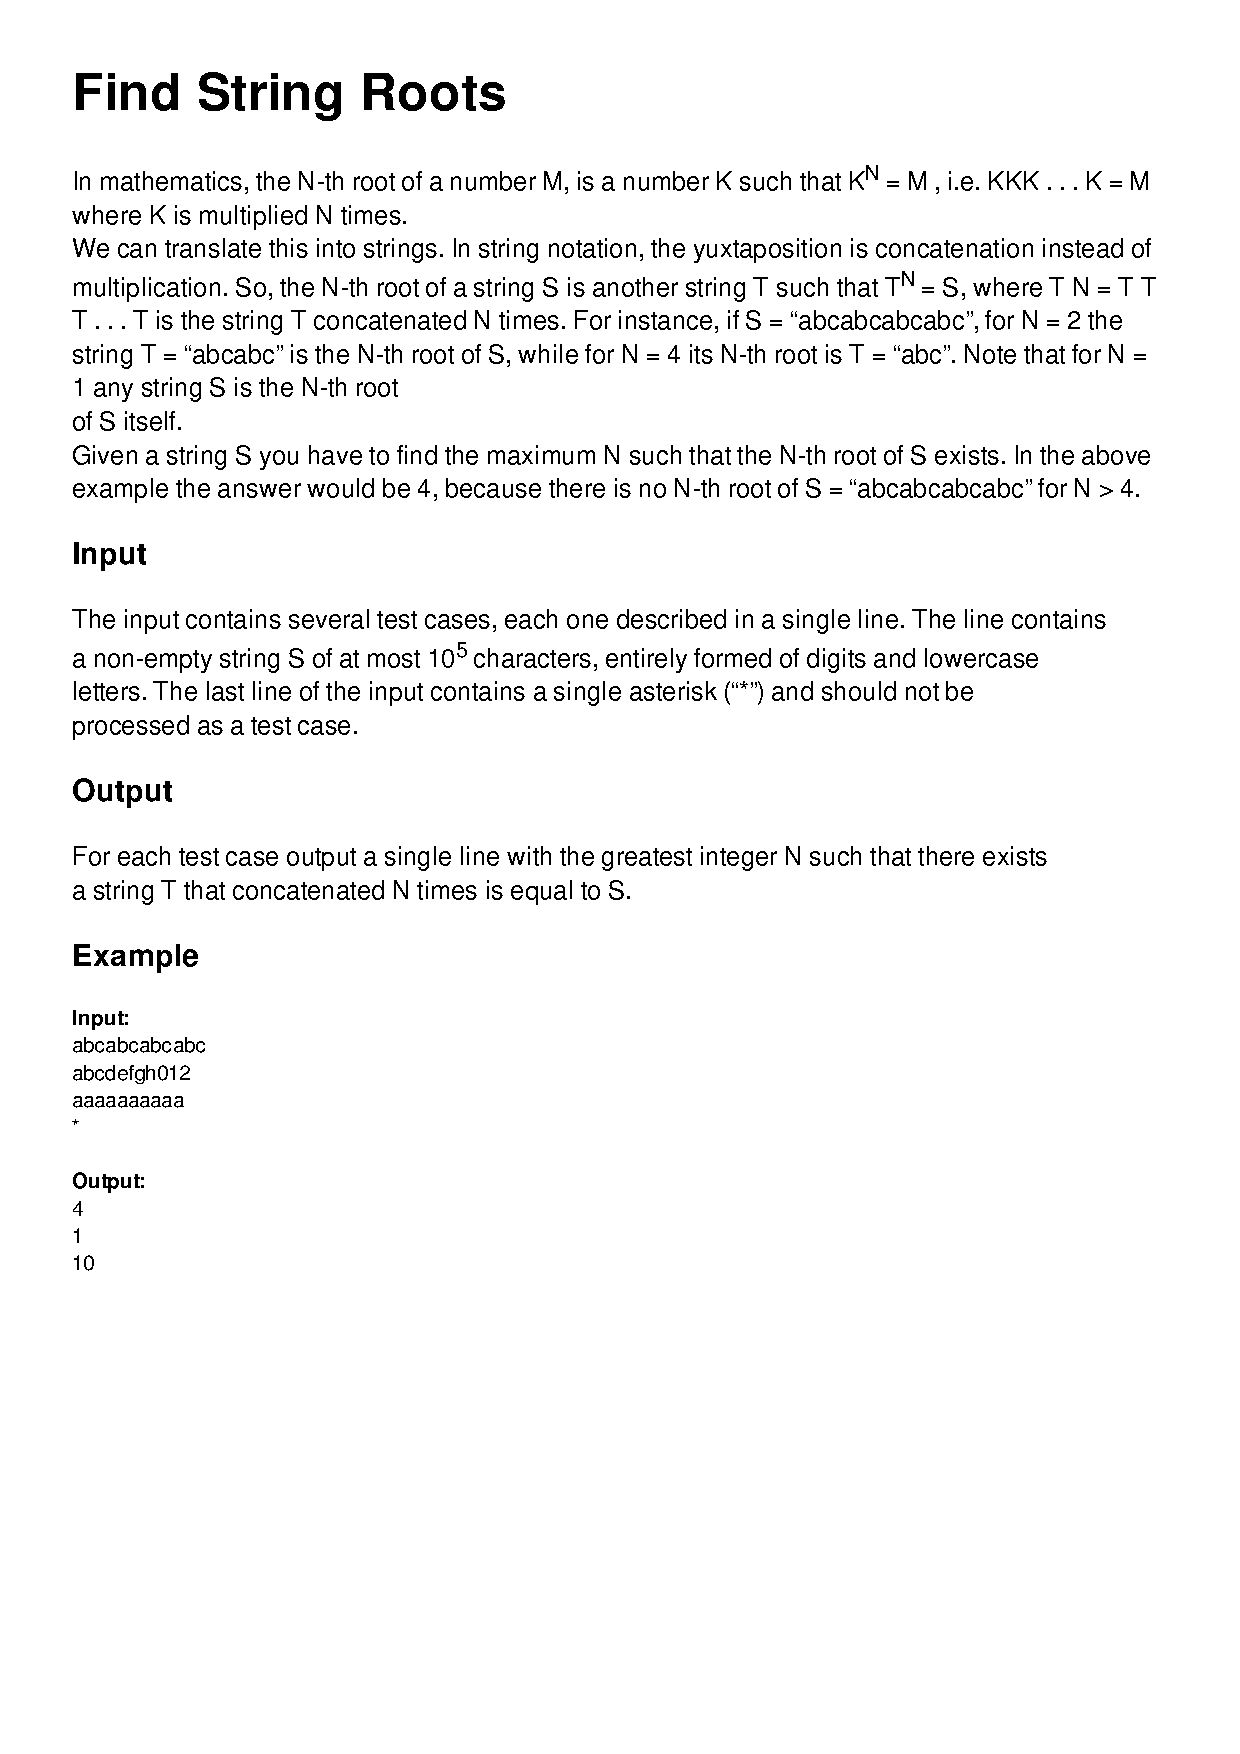
\includepdf[pages=-]{problemas/pdf/FINDSR.pdf}

\subsubsection{Análisis}
Como se había dicho previamente, ya se había atacado este problema así que se omitirá el análisis
y la complejidad.

\subsubsection{Entrada}
Una \textit{heurística} a seguir es que siempre que diga: \textit{``the input contains several test
cases, each line described in a single line''} es leer hasta el final de archivo (End Of File) cada
línea. Seguido de esto, dice que cada línea una cadena no vacía de a lo más $10^5$
caracteres\footnote{Hay lenguajes programación que no tienen implementadas cadenas, y que se debe
saber de antemano el tamaño, para así tener un arreglo de $n$ caracteres. Es aquí cuando es
importante saber el tamaño máximo de la entrada.} formada solamente de dígitos y letras en
minúsculas\footnote{También es sumamente importante saber si las cadenas del lenguaje que se usará
como son represntadas ya que podrían estar en ASCII o Unicode.}.
Finalmente dice que la última entrada contiene un solo asterisco \texttt{*} y que no debe ser
procesado como un caso más.

\subsubsection{Salida}
Para cada caso prueba \textit{(input)} se debe imprimir en la salida estándar una sola línea con un
número $n$ siendo ésta la raíz de la cadena, es decir, el número de veces que está concatenada la
cadena consigo misma.

\subsubsection{Ejemplos}
\begin{itemize}
\item Consideremos la entrada $x =$ \texttt{abcabcabcabc} y sobre ésta se construye la función
de error, 
\begin{table}[h]
\centering
\begin{tabular}{c|c|c|c|c|c|c|c|c|c|c|c|c|}
\cline{2-13}
$i$      & 1          & 2          & 3          & 4          & 5          & 6          & 7          & 8          & 9          & 10         & 11         & 12         \\ \hline
$P[i]$   & \texttt{a} & \texttt{b} & \texttt{c} & \texttt{a} & \texttt{b} & \texttt{c} & \texttt{a} & \texttt{b} & \texttt{c} & \texttt{a} & \texttt{b} & \texttt{c} \\ \hline
$\pi[i]$ & 0          & 0          & 0          & 1          & 2          & 3          & 4          & 5          & 6          & 7          & 8          & 9          \\ \cline{2-13} 
\end{tabular}
\end{table}

Siendo $\vert x \vert = 12$ y el último elemento de la función de error es $\pi[m] = 9$ y sea
$r = 12 - 9 = 3$. Se conluye que la raíz de la cadena es de longitud \textbf{3} y su factor de
repetición es $\rho(x) = \frac{12}{3} =$ \textbf{4}. Concluyendo así que
\texttt{(abc)}$^4 = $ \texttt{abcabcabcabc}.

\item Consideremos la entrada $x =$ \texttt{acbdefgh012} y sobre ésta se construye la función
de error, 
\begin{table}[h]
\centering
\begin{tabular}{c|c|c|c|c|c|c|c|c|c|c|c|}
\cline{2-12}
$i$      & 1          & 2          & 3          & 4          & 5          & 6          & 7          & 8          & 9          & 10         & 11         \\ \hline
$P[i]$   & \texttt{a} & \texttt{b} & \texttt{c} & \texttt{d} & \texttt{e} & \texttt{f} & \texttt{g} & \texttt{h} & \texttt{0} & \texttt{1} & \texttt{2} \\ \hline
$\pi[i]$ & 0          & 0          & 0          & 0          & 0          & 0          & 0          & 0          & 0          & 0          & 0          \\ \cline{2-12} 
\end{tabular}
\end{table}

Siendo $\vert x \vert = 11$ y el último elemento de la función de error es $\pi[m] = 0$ y sea
$r = 11 - 0 = 11$. Teniendo que su factor de repetición es $\rho(x) = $ \textbf{1}. Concluyendo
así que\texttt{(acbdefgh012)}$^1 = $ \texttt{acbdefgh012}.

\item Consideremos la entrada $x =$ \texttt{aaaaaaaaaa} y sobre ésta se construye la función
de error, 
\begin{table}[h]
\centering
\begin{tabular}{c|c|c|c|c|c|c|c|c|c|c|}
\cline{2-11}
$i$      & 1          & 2          & 3          & 4          & 5          & 6          & 7          & 8          & 9          & 10         \\ \hline
$P[i]$   & \texttt{a} & \texttt{a} & \texttt{a} & \texttt{a} & \texttt{a} & \texttt{a} & \texttt{a} & \texttt{a} & \texttt{a} & \texttt{a} \\ \hline
$\pi[i]$ & 0          & 1          & 2          & 3          & 4          & 5          & 6          & 7          & 8          & 9          \\ \cline{2-11} 
\end{tabular}
\end{table}

Siendo $\vert x \vert = 10$ y el último elemento de la función de error es $\pi[m] = 9$ y sea
$r = 10 - 9 = 1$. Se conluye que la raíz de la cadena es de longitud \textbf{1} y su factor de
repetición es $\rho(x) = \frac{10}{1} =$ \textbf{1}. Concluyendo así que
\texttt{(a)}$^{10} = $ \texttt{aaaaaaaaaa}.
\end{itemize}
\newpage

\subsubsection{Implementación en C++}
\inputminted[linenos, frame=lines, fontsize=\footnotesize]{cpp}{problemas/cpp/FINDSR.cpp}

\begin{itemize}
\item En la línea \texttt{1} se agrega la cabecera \texttt{iostream} que define la entrada y salida
estándar. En la línea \texttt{2} se agrega la cabecera \texttt{vector} que son contenedores de
arreglos dinámicos.

\item De línea \texttt{6} a \texttt{19} es la implementación de la función de error.

\item En la línea \texttt{23} es la parte importante sobre leer la entrada; se leerá hasta EOF y si
la cadean leída es diferente de \texttt{*}.

\item En la línea \texttt{24} se crea un vector con la función de error con el patrón \texttt{s}, y
en la línea \texttt{28} se obtiene la posible longitud de la $k$-ésima raíz del patrón.

\item Y de la línea \texttt{30} a \texttt{33} es cuando se hace la validación previamente analizada.
\end{itemize}

\subsubsection{Implementación en Haskell}
\inputminted[linenos, frame=lines]{haskell}{problemas/haskell/FINDSR.hs}

\begin{itemize}
\item En la línea \texttt{1} del módulo \hsCode{Data.Array} importamos solamente el tipo
\hsCode{Array} sin ninguno de sus constructores, la función \hsCode{bounds :: Array i e -> (i, i)}
que devuelve los límites del arreglo en cual fue construido,\\
\hsCode{listArray :: Ix i => (i, i) -> [e] -> Array i e} que construye un arreglo donde el primer
argumentos son los límites inferiores y superiores, y una lista de valores devolviendo valores
con un orden indexado,\\
\hsCode{(!) :: Ix i => Array i e -> i -> e}  regresa el valor de un índice dado en el arreglo.

\item Analicemos parte por partes las líneas \texttt{3, 4}. recordemos la función \\
\hsCode{interact :: (String -> String) -> IO ()}, la función \hsCode{interact} toma una función de
tipo \hsCode{(String -> String)} como argumento. La \textit{entrada} entera de la entrada estándar
es pasada a ésa función como argumento, y la cadena resultante es la \textit{salida} de la
salida estándar.

Acto seguido, se tiene la función \texttt{\$} que es un operador infijo con asociatividad izquierda,
esto para tener mejor legibilidad cuando se tienen argumentos largos.

Dado que se procesará linea por línea de la entrada, es bastante común tratar el flujo de la
entrada como una lista de líneas, así que para hacer eso se divirá todo la cadena de entrada en
líneas. Consideremos las funciones\\ \hsCode{lines :: String -> [String]} y
\hsCode{unlines :: [String] -> String}, donde\\ \hsCode{lines} divide la cadena en una lista de
cadenas cuando se encuentra un caracter de salto de línea, \hsCode{unlines} es la operación inversa
de \hsCode{lines}, une líneas y después añade un caracter de salto de línea a cada cadena.

Pongamos total atención a la siguiente composición de funciones\\
\hsCode{unlines . map parse . takeWhile (/= "*") . lines}.\\
La función \hsCode{map parse} será la responsable de que la cadena en turno la tranformará a la
respuesta del problema.

La función \hsCode{takeWhile :: (a -> Bool) -> [a] -> [a]}, aplicado a un predicado \hsCode{p} y
una lista \texttt{xs}, regresa el prefijo más largo (que posiblemente puede ser vacío) de
\texttt{xs} de los elemetos que satisfacen \hsCode{p}.
Entonces \hsCode{takeWhile (/= "*")} significa que se seguirá procesanso hasta que la cadena leída
sea diferente de \texttt{*}.

El patrón \hsCode{unlines . f . lines} es un patrón bastamte común donde \hsCode{f} puede ser una
función o composición de funciones donde \hsCode{f :: [String] -> [String]}.

\item De la línea \texttt{6, 7} la función \hsCode{parse} será la responsable de tomar la cadena en
turno, tomar el resultado de \hsCode{process} y convertirlo al tipo \hsCode{String}.

En el punto siguiente se hablará sobre la función \hsCode{process :: String -> Int}, pero básicamente es
la que ``hará el algoritmo'', lo importame aquí es el tipo \hsCode{Int}, y es por eso que se hizo
la función \hsCode{parse :: String -> String}.

\item De igual manera de las líneas \texttt{8} a \texttt{16} en la expresión \hsCode{let ... in ...}
en la línea \texttt{10} se calcula la función de error de la cadena de entrada, en la \texttt{11}
se obtienen los límites del arreglo siendo la segunda entrada tamaño del arreglo, y en la línea
\texttt{12} se obtiene el último elemento del arreglo y después su índice. En la línea \texttt{13}
se obtiene la posible longitud de la $k$-ésima raíz del patrón. Finalmente de la línea \texttt{14}
a \texttt{16} es cuando se hace la validación previamente analizada.

\item De la línea \texttt{19} a \texttt{29} es la implementación de función de error.
\end{itemize}

\subsubsection{Resultado del juez}
\begin{figure}[H]
\centering
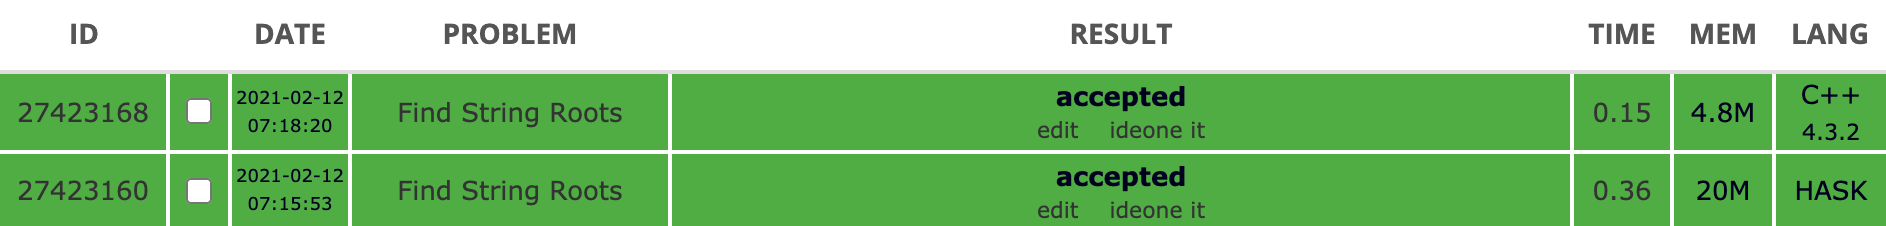
\includegraphics[width=\textwidth]{spoj/FINDSR-accepted-cpp-haskell}
\caption{El código fue aceptado por el juez en Haskell y C++}
\end{figure}

\newpage


\subsection{Ver si una cadena es una rotación cíclica de otra}

\subsubsection{Análisis}
De igual manera, el en \hyperlink{cyclic_rotation}{capítulo 3 el problema 32.4-7} se había hecho el
análisis del problema, y como este problema es resovler exactamente lo mismo se omitirá el análisis
y su complejidad.

\subsubsection{Entrada}
Este tipo de entrada es la más común que se verá en la programación competitiva; ya que la primera
línea será un entero con el número de casos a resolver, después caso consistirá de dos líneas.

Igual que el problema anterior (e igual que en la mayoría de los problemas de este índole) la
entrada será sobre un alfabeto de \texttt{[a-z]} entonces serán representados en ASCII.

\subsubsection{Salida}
Solo se deberá mostrar en la salida estándar \texttt{Si} o \texttt{No} dependiendo si es una
rotación cíclica.

\subsubsection{Ejemplos}
Dado que ambas cadenas son de la misma longitud se hará lo siguiente, $s = qq$ donde $s$ será el
texto y $p$ el patrón. Entonces con el algoritmo dee Knuth-Morris-Pratt se buscará $p$ en $s$.

\begin{itemize}
\item \texttt{abc} es una rotación cíclica de \texttt{cab} porque \texttt{cab} $\mapsto$
\texttt{abc}. Se muestra en la siguiente tabla de manera gráfica la idea.
\begin{table}[h]
\centering
\begin{tabular}{|c|c|c|c|c|c|}
\hline
\texttt{c}                   &  \cellcolor{green}\texttt{a} &  \cellcolor{green}\texttt{b} &
\cellcolor{green} \texttt{c} &  \texttt{a}                  & \texttt{b}                   \\\hline
\end{tabular}
\end{table}

\item Claramente \texttt{abab} no es rotación cíclica de \texttt{aabb}.
\begin{table}[h]
\centering
\begin{tabular}{|c|c|c|c|c|c|c|c|}
\hline
\texttt{a} & \texttt{b} & \texttt{a} &\texttt{b} & \texttt{a} & \texttt{b} & \texttt{a} & \texttt{b} \\\hline
\end{tabular}
\end{table}
\end{itemize}

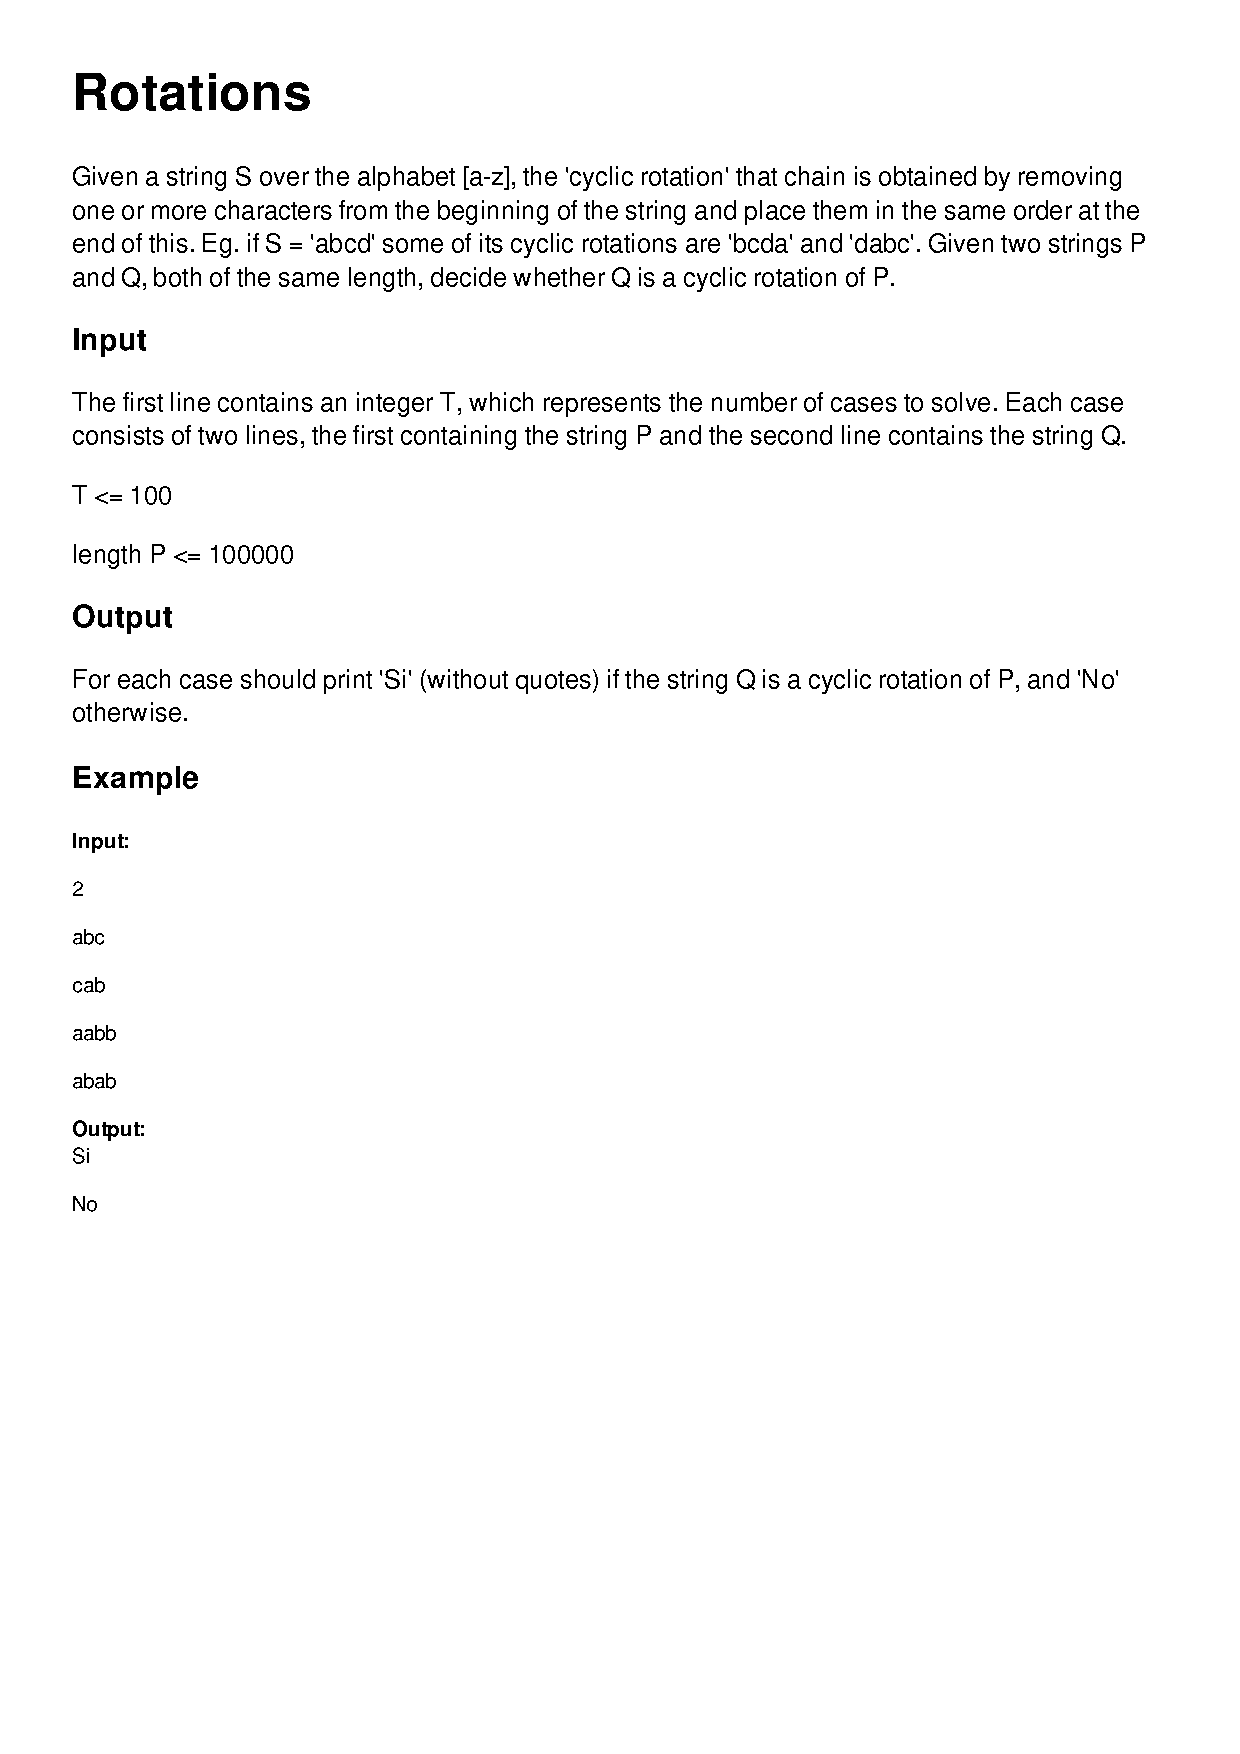
\includepdf[pages=-]{problemas/pdf/EC_WORLD.pdf}

\subsubsection{Implementación en C++}
\inputminted[linenos, frame=lines, fontsize=\footnotesize]{cpp}{problemas/cpp/EC_WORLD.cpp}
\begin{itemize}
\item a
\end{itemize}

\subsubsection{Implementación en Haskell}
% TODO: poner que este problema no lo acepta el juez
\inputminted[linenos, frame=lines, fontsize=\small]{haskell}{problemas/haskell/EC_WORLD.hs}
\begin{itemize}
\item a
\end{itemize}

\subsubsection{Resultado del juez}
\begin{figure}[h]
\centering
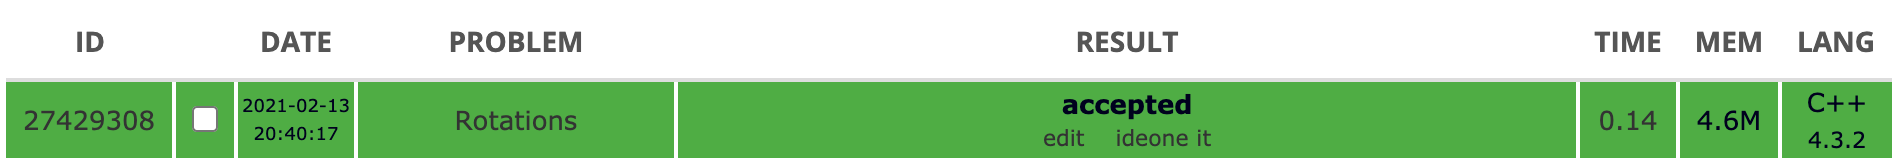
\includegraphics[width=\textwidth]{spoj/EC_WORLD-accepted-cpp}
\caption{El código fue aceptado por el juez en C++}
\end{figure}

\newpage


\subsection{Extender una cadena a un palíndromo}

\subsubsection{Análisis}

\subsubsection{Entrada}

\subsubsection{Salida}

\subsubsection{Ejemplos}
\begin{itemize}
\item a
\item a
\item a
\item a
\end{itemize}

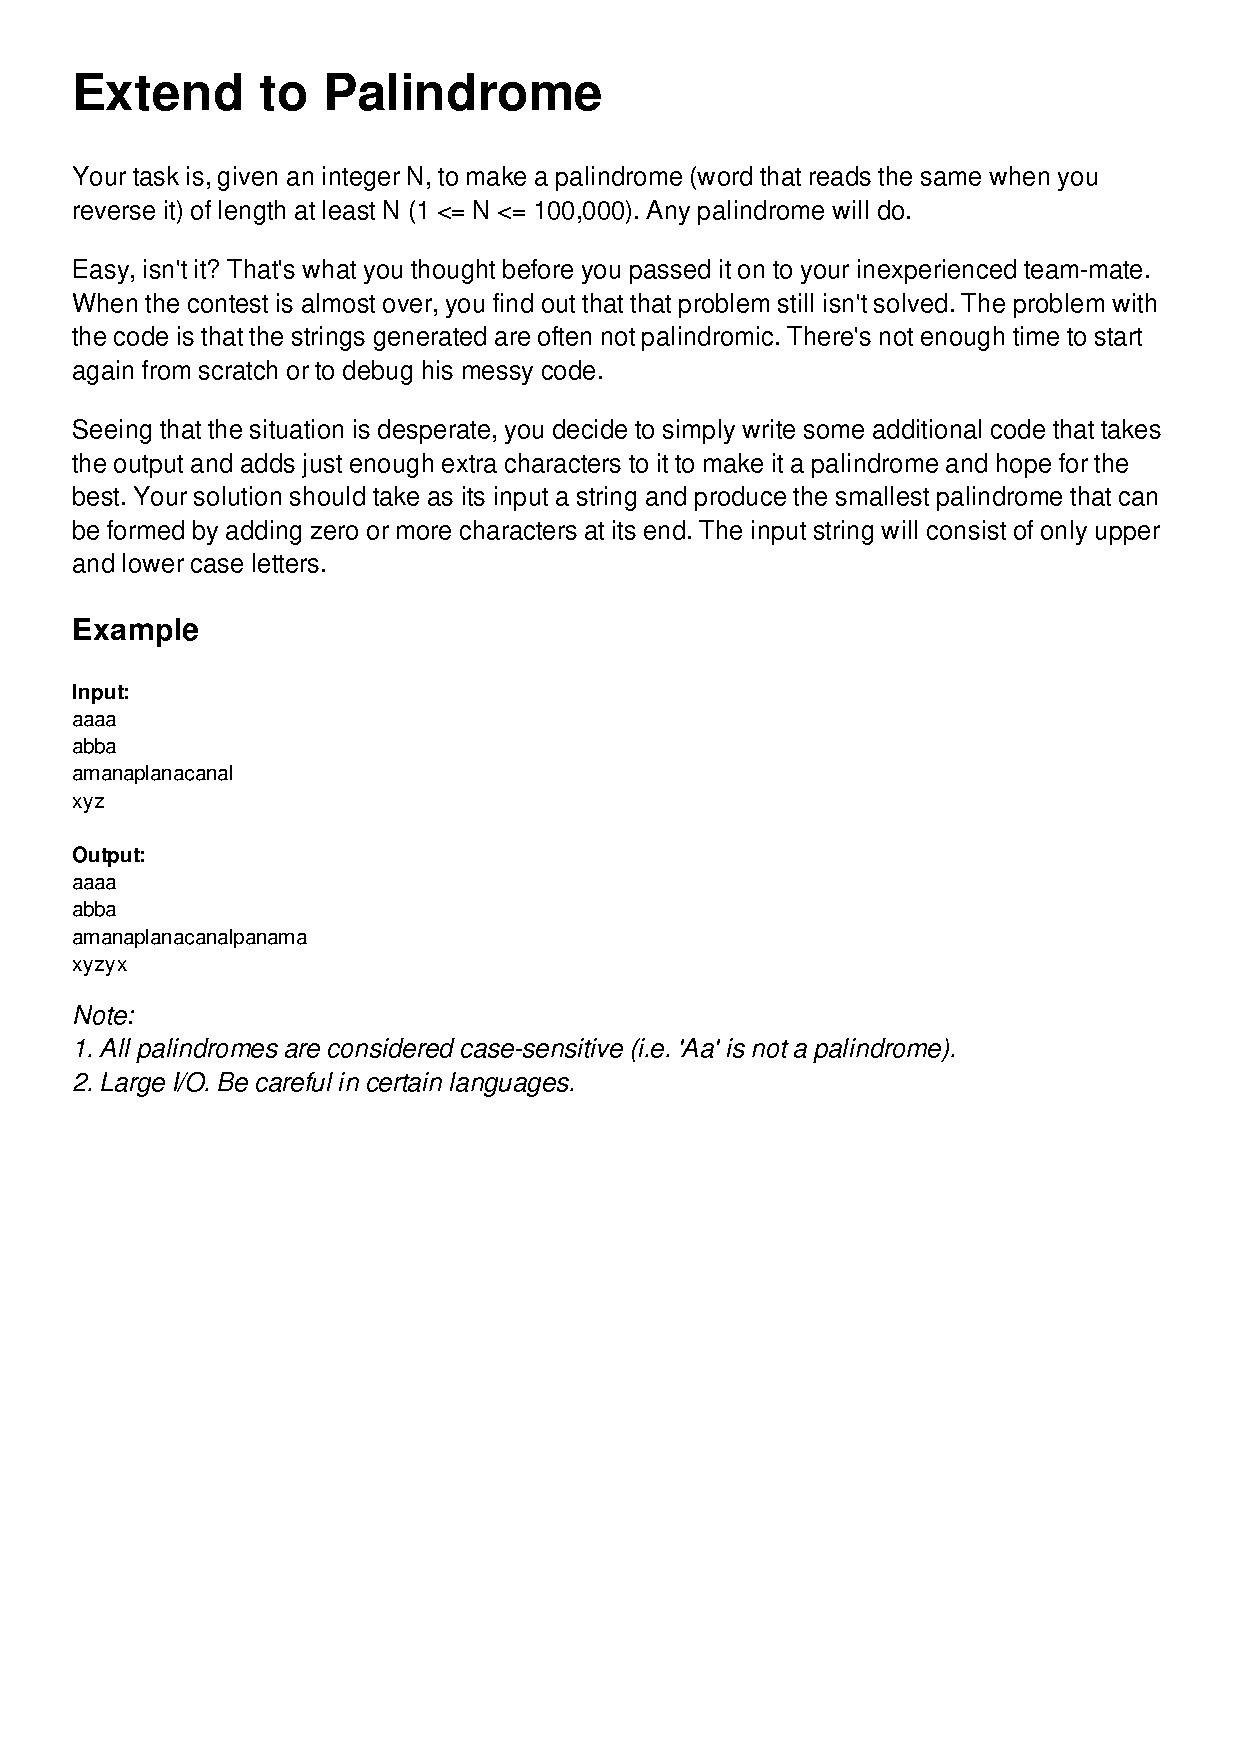
\includepdf[pages=-]{problemas/pdf/EPALIN.pdf}

\subsubsection{Implementación en C++}
\inputminted[linenos, frame=lines]{cpp}{problemas/cpp/EPALIN.cpp}

\begin{itemize}
\item a
\end{itemize}

\subsubsection{Implementación en Haskell}
\inputminted[linenos, frame=lines]{haskell}{problemas/haskell/EPALIN.hs}

\begin{itemize}
\item a
\end{itemize}

\subsubsection{Resultado del juez}
\begin{figure}[h]
\centering
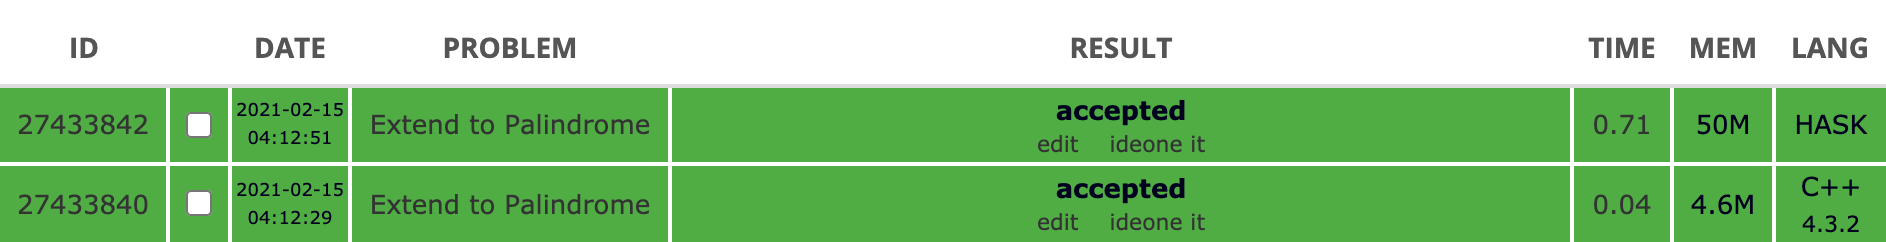
\includegraphics[width=\textwidth]{spoj/EPALIN-accepted-cpp-haskell}
\caption{El código fue aceptado por el juez en Haskell y C++}
\end{figure}

\newpage


\subsection{Encontrar todas las ocurrencias de un patrón en un texto}

\subsubsection{Análisis}

\subsubsection{Entrada}

\subsubsection{Salida}

\subsubsection{Ejemplos}
\begin{itemize}
\item a
\item a
\item a
\item a
\end{itemize}

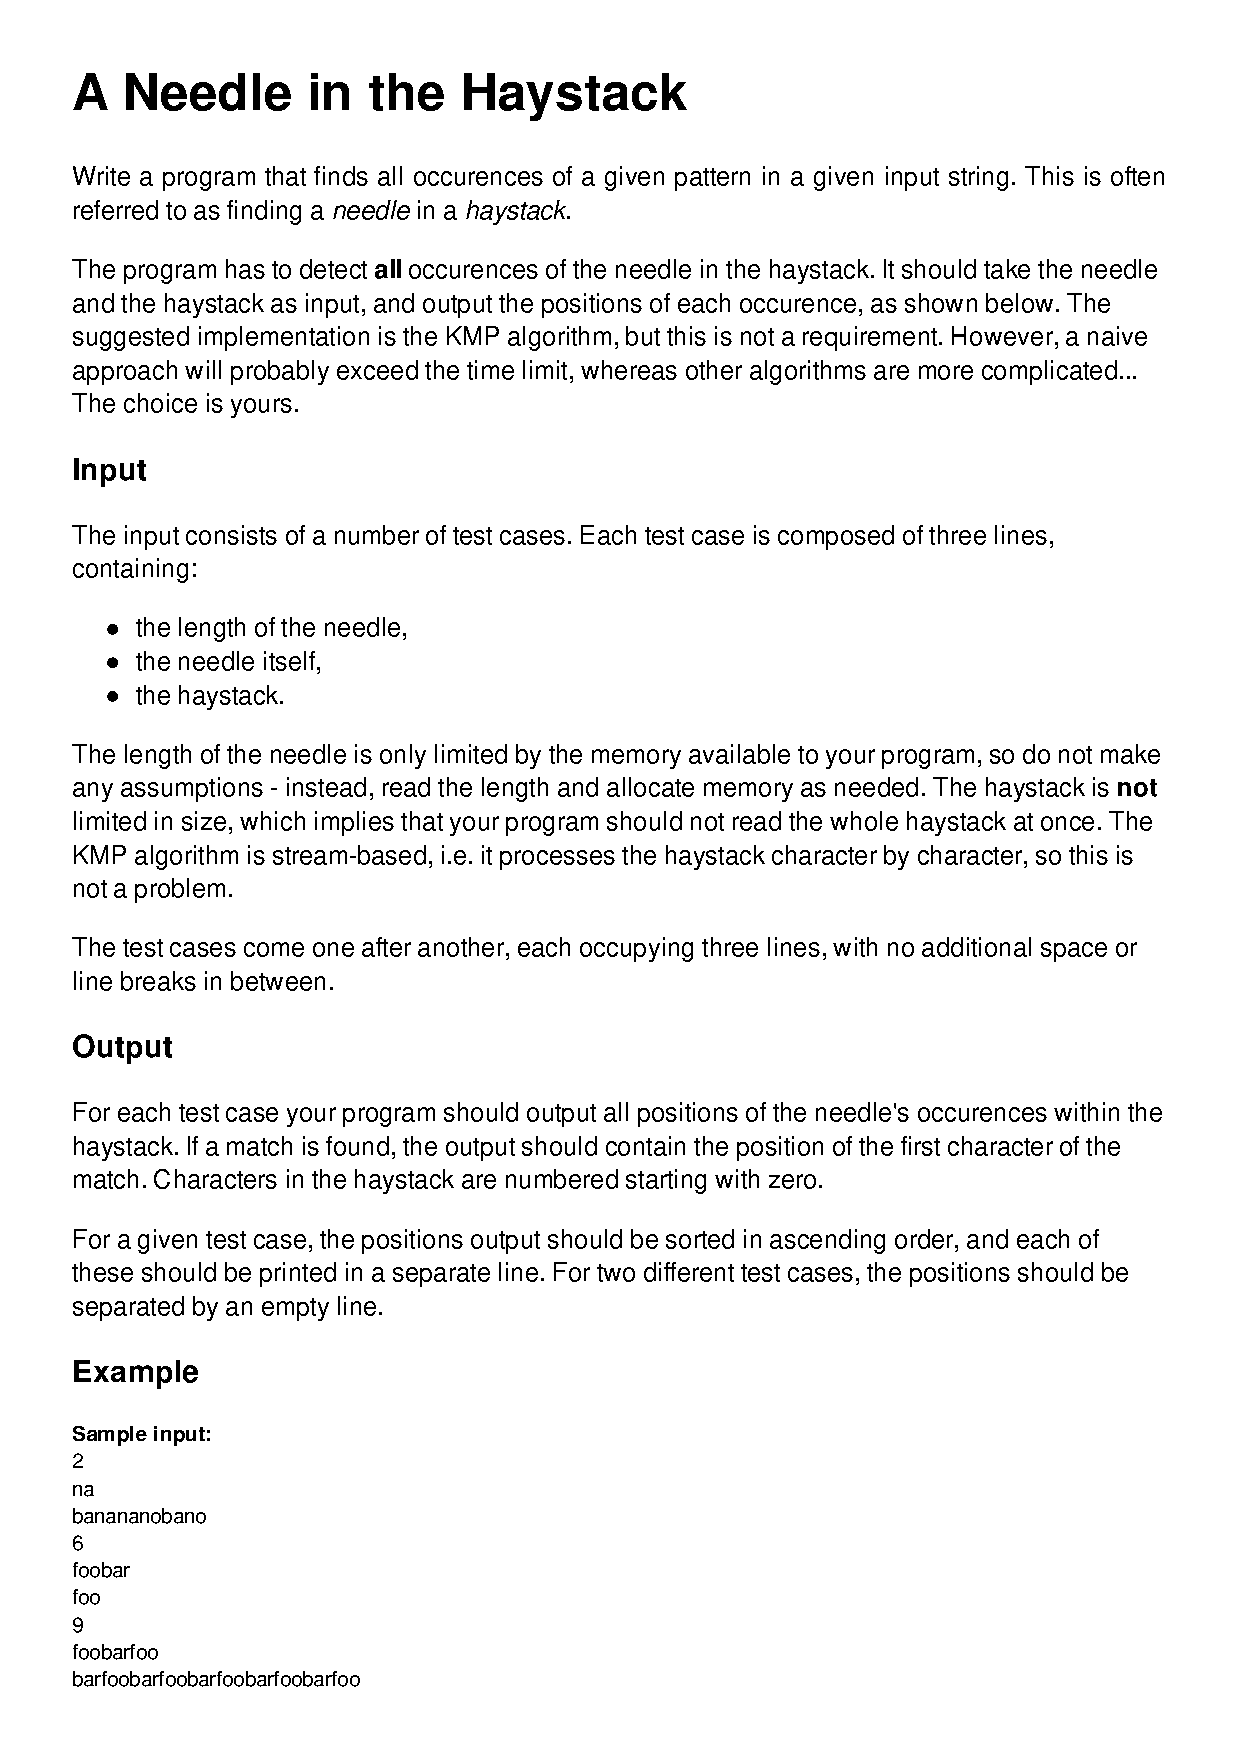
\includepdf[pages=-]{problemas/pdf/NHAY.pdf}

\subsubsection{Implementación en C++}
\inputminted[linenos, frame=lines]{cpp}{problemas/cpp/NHAY.cpp}

\begin{itemize}
\item a
\end{itemize}

\subsubsection{Implementación en Haskell}
\inputminted[linenos, frame=lines]{haskell}{problemas/haskell/NHAY.hs}

\begin{itemize}
\item a
\end{itemize}

\subsubsection{Resultado del juez}
\begin{figure}[h]
\centering
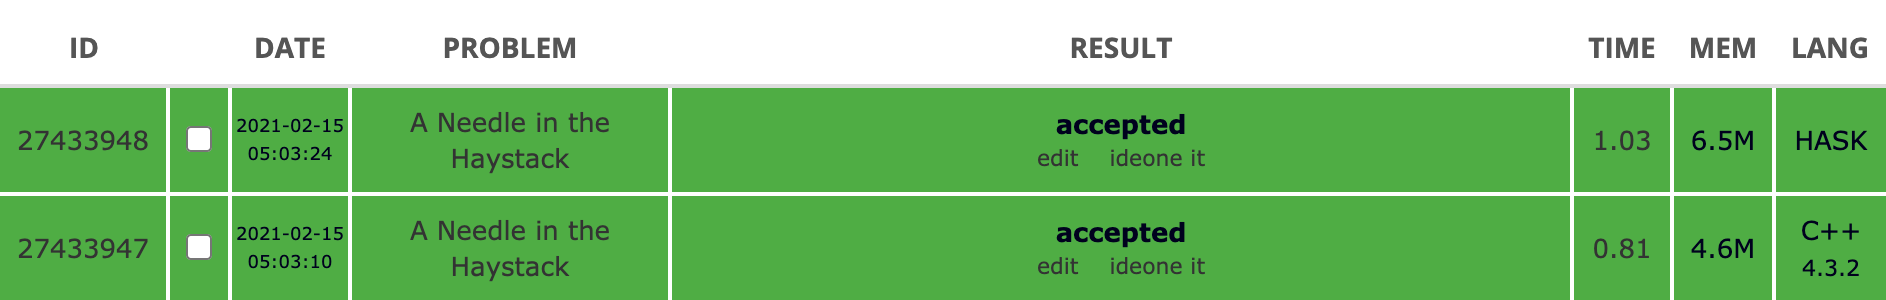
\includegraphics[width=\textwidth]{spoj/NHAY-accepted-cpp-haskell}
\caption{El código fue aceptado por el juez en Haskell y C++}
\end{figure}
% TODO: Chane y justifico esto el <$> https://ro-che.info/articles/2019-07-22-associativity-of-fmap



% TODO: poner que puedo optimizar la entrada con Data.ByteString.Char8

    \chapter{Benchmarks}
        \input{capitulos/10-benchmarks}
    
    \chapter{Conclusiones}
        \lipsum[1-4]



\backmatter
    \nocite{*}
    \printbibliography

\end{document}
